\newpage
\GpSec{Architektur}\label{sec:architecureflutter}
\subsection{Ordnerstruktur }\label{Ordnerstruktur}
 \begin{verbatim}
|---assets
    |---fonts
    |---images
|---lib
    |---(Client/Admin/Login Sicht)
        |---config
            |---properties
        |---domain
            |---persistent
            |---exception
        |---pages
            |---navigation
            |---settings
            |---....
            |---widgets
                |---widget
                |---...
        |---provider
            |---rest
                |---dtos
            |---theme
\end{verbatim}
{\bf{Anmerkung}:} Dieser Aufbau beschreibt die generelle Struktur für die Admin-, Client- und Login Sicht. Jede Sicht implementiert diese Architektur


\begin{itemize}
    \item \textbf{assets}: Enthält selbst hinzugefügte Dateien, die für die Ausführung der Applikation notwendig sind. Assets umfassen verschiedene Arten von Informationen wie: Bilder, Schriftarten, Musik, Umgebungs-Informationen, usw.
    \item \textbf{lib}: Dieser Ordner enthält den gesamten Quellcode der Anwendung.
    \item \textbf{config}: Enthält statische Informationen wie Farben, URLs, usw. 
    \item \textbf{domain}: Dieser Ordner umfasst die Funktionalität bzw. Business-Logik. Ebenfalls enthalten ist der Ordner {\textit persistent}, der für die Speicherung bzw. Verwaltung von Daten zuständig ist. Der Ordner {\textit{Exception}} beinhaltet die selbst erstellen Exceptions
    \item \textbf{pages}: Umfasst alle Seiten, die je nach Sicht benötigt werden. Auch hier befindet sich der Ordner {\textit widgets}, der Widgets enthält, die in den verschiedenen Ansichten mehrmals verwendet werden.
    \item \textbf{provider}: Ist für die Zustandsverwaltung der App zuständig. In unserem Fall befindeen sich dort hauptsächlich die API-Verbindungen sowie die Verwaltung des \ref{subsec:impl:themehandler} \nameref{subsec:impl:themehandler}.
    \begin{itemize}
        \item Der Ordner {\textit{rest}} beinhaltet, den Ordner {\textit{Dtos}} (Data Transfer Objects), welcher die verschiedenen Klassen zur Deserialisierung der API Daten enth\"alt
    \end{itemize}
\end{itemize}
\newpage

\subsection{Trennung der Schichten }\label{subsec:seperationlayers}

\begin{figure}[h!]
\centering
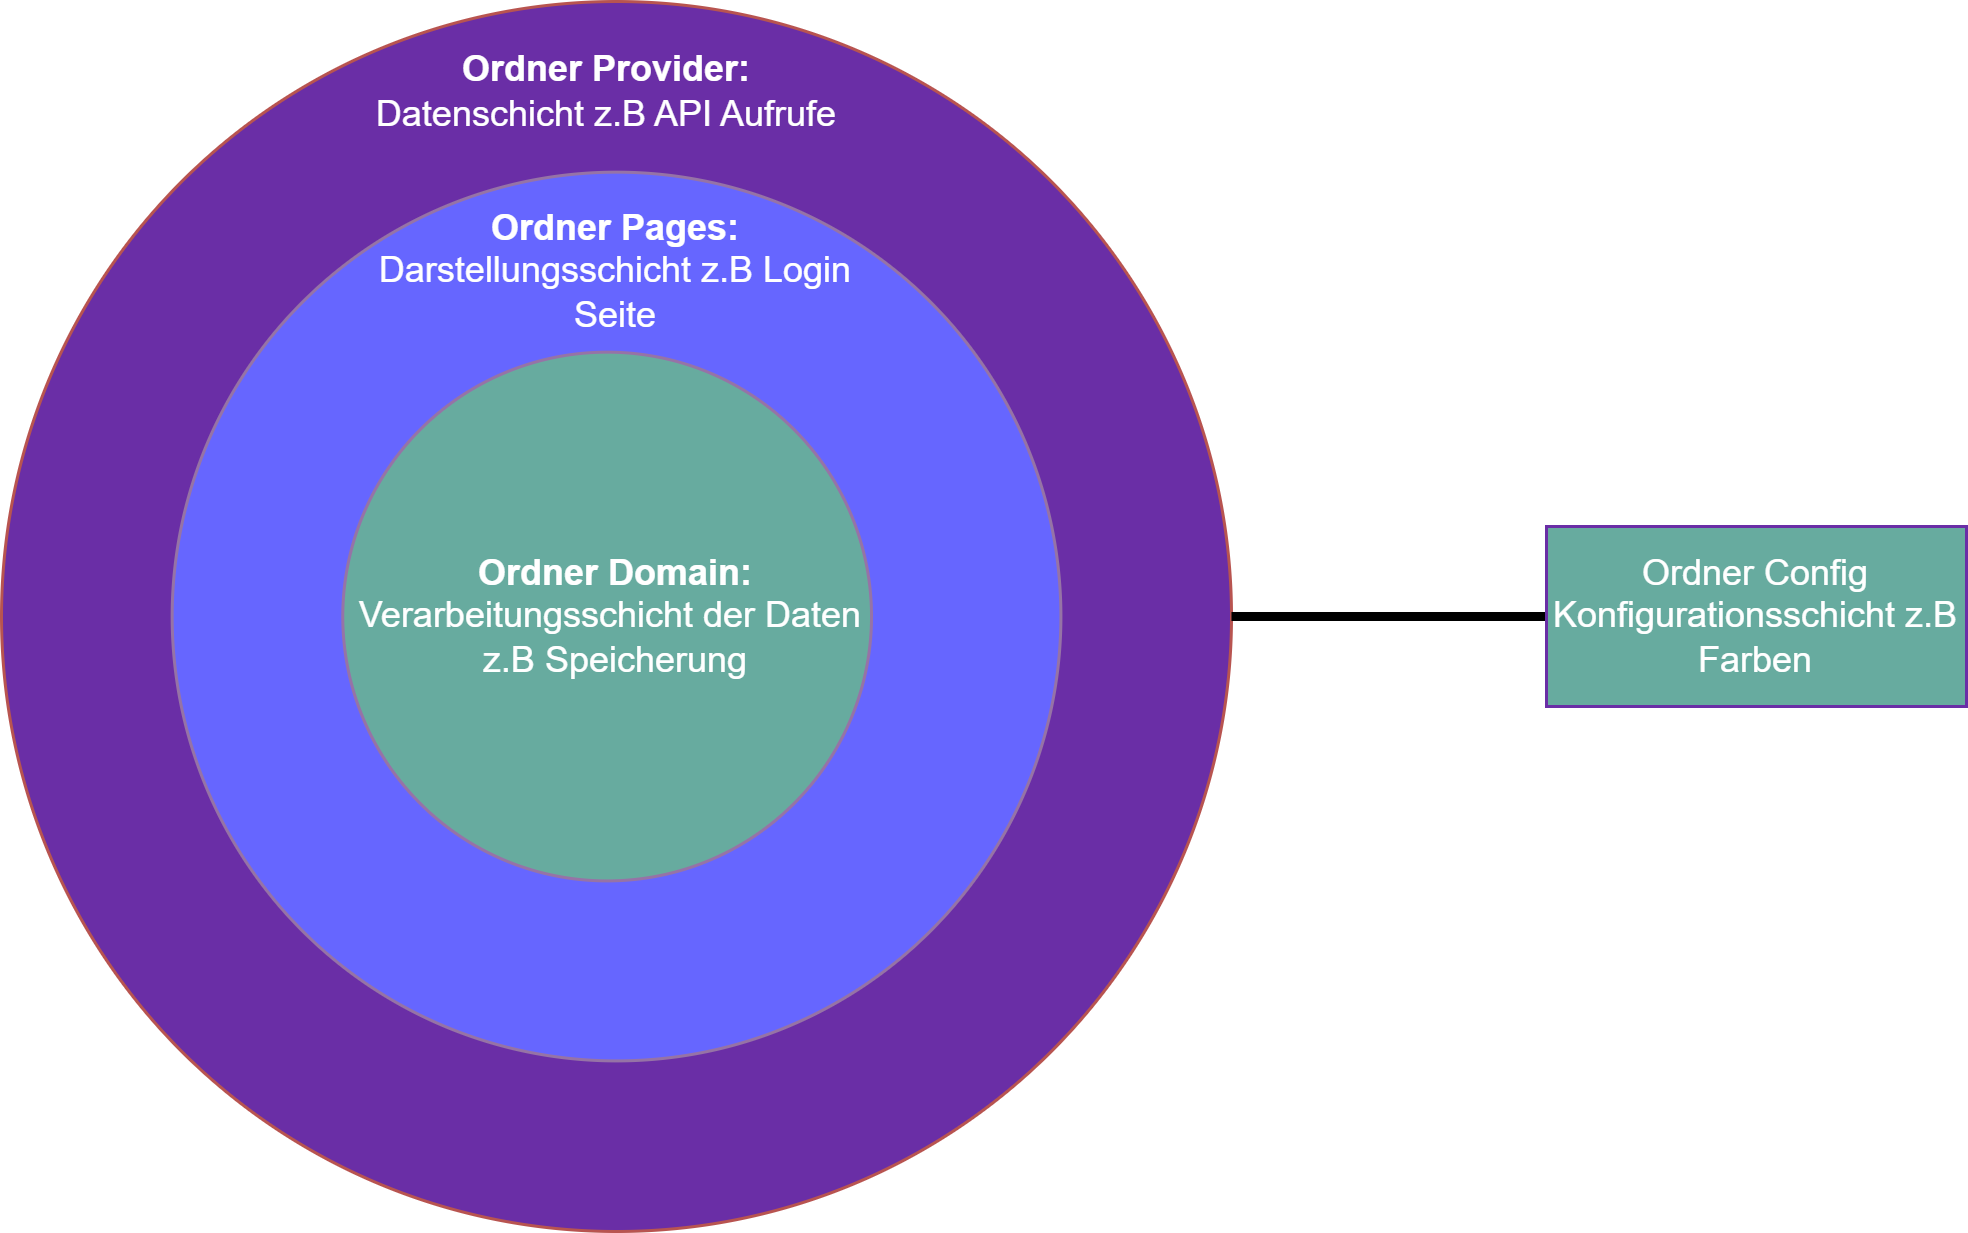
\includegraphics[width=0.9\textwidth]{FLUTTER/images/GP/layers.png}
\caption{Grafische Darstellung der Schichten (vgl. \cite{flutter-layer})}
\end{figure}

Die Trennung der Anwendungslogik, Präsentationslogik und der Darstellungsschicht in der Entwicklung einer Anwendung bietet folgende Vorteile: (vgl. \cite{flutter-layer})
\begin{itemize}
    \item {\textbf{Flexibilität}}: Durch die Aufteilung in unabhängige Schichten, ist es möglich, jede Schicht ohne Auswirkungen auf eine andere zu verändern. Dies ist vor allem bei Änderungen der Benutzeroberfläche nützlich, da die Logik der zugrundeliegenden Schicht nicht verändert werden muss.
    \item {\textbf{Wiederverwendbarkeit}}: Da die Schichten unabhängig voneinander sind, können Teile der Anwendung in anderen Applikationen verwendet werden
    \item {\textbf{Testbarkeit}}: Es ist möglich, jede Schicht einzeln zu testen, was zu einer schnelleren Fehlerbehandlung führt
    \item {\textbf{Erweiterbarkeit}}: Es ist um ein Vielfaches einfacher, eine Schicht zu erweitern, wenn die zugrunde liegende Schicht nicht mit verändert werden muss.
\end{itemize}
Durch die Trennung der Schichten, wird eine gute Basis, für die Weiterentwicklung bzw. das Verständnis des Programmes ermöglicht.

\section{Spezialit\"aten}
\ZbSSec{pubspec.yaml }\label{pubspec.yaml}
Das {\textit {pubspec.yaml}} ist die Konfigurationsdatei, welche für das Definieren der Metadaten eines Flutter Projektes verantwortlich ist. Es beinhaltet wichtige Informationen wie: verwendete Bibliotheken, SDK-Version, usw. Im nachfolgenden Abschnitt wird das verwendete {\textit {pubspec.yaml}} beschrieben. \\
{\textbf {Hinweis}:} Das verwendete {\textit {pubspec.yaml}} ist nicht unter {\textit {/assets}} aufzufinden, da das Flutter-Framework den Speicherort des Files am äußersten Ordner des Projektes vorgibt.\\ {\bf{Anmerkung}:} Die spezifischere Erklärung bzw. Verwendung der einzelnen Pakte wird im Laufe des restlichen Dokumentes genauer beschrieben.
\newpage
\begin{lstlisting}[caption={Konfigurationdatei pubspec.yaml},style=goMono]
name: card\_master
description: A Flutter app for our diploma thesis about a card storage management system.

publish\_to: 'none' # Remove this line if you wish to publish to pub.dev

# The following defines the version and build number for your application.
version: 1.0.0+1
environment:
  sdk: '>=2.18.5 <3.0.0'

# Dependencies specify other packages that your package needs in order to work.
dependencies: 
  flutter:
    sdk: flutter
  cupertino_icons: ^1.0.2
  web_socket_channel: ^2.3.0
  provider: ^6.0.5
  shared_preferences: ^2.0.17
  flutter_dotenv: ^5.0.2
  flutter_secure_storage: ^5.0.2
  flutter_local_notifications: ^9.6.0
  rxdart: ^0.27.7
  app_settings: ^4.2.0
  open_mail_app: ^0.4.5
  intl: ^0.17.0
  awesome_snackbar_content: ^0.1.0
  flutter_datetime_picker: ^1.5.1
  tuple: ^2.0.1
  aad_oauth: ^0.4.0
  charts_flutter: ^0.12.0

dev\_dependencies:
  flutter_test:
    sdk: flutter
  flutter_lints: ^2.0.0
flutter:
  assets:
    - .env
    - img/
    - azure.env
  fonts:
    - family: Kanit
      fonts: ....
\end{lstlisting}

\newpage

\begin{itemize}
    \item \textbf{publis.to}: Gibt an, ob das Projekt als Paket im Internet zur Verfügung gestellt werden soll.
    \item \textbf{enviroment}: Die notwendige Version der Entwicklungsumgebung Flutter
    \item \textbf{dependencies}: Beschreibt die verwendeten Pakete.
    \begin{itemize}
        \item \textbf{cupertino\_icons}: Icons für IOS-Apps
        \item \textbf{web\_socket\_channel}: Für die Verwendung von Websockets
        \item \textbf{provider}: Zustandsmanagement Framework, welches hauptsächlich für den \ref{subsec:impl:themehandler} \nameref{subsec:impl:themehandler}  verwendet wird 
        \item \textbf{shared\_preferences}: Dient zur Speicherung von Daten am Gerät
        \item \textbf{flutter\_dotenv}: Wird verwendet, um Umgebungsvariablen in der Applikation zu verwalten
        \item \textbf{flutter\_secure\_storage}: Dient zur sicheren Speicherung von Daten am Gerät
        \item \textbf{flutter\_local\_notifications}: Wird verwendet, um Benachrichtigungen am Gerät zu versenden
        \item \textbf{rxdart}: Für asynchrone Programmierung
        \item \textbf{app\_settings}: Wird verwendet, um die Einstellung am Gerät zu öffnen
        \item \textbf{open\_mail\_app}: Wird verwendet, um Mail-Apps zu öffnen
        \item \textbf{intl}: Wird von Flutter benötigt
        \item \textbf{awesome\_snackbar\_content}: Wird zur Erstellung von Pop-Up verwendet
        \item \textbf{flutter\_datetime\_picker}: Wird für das Reservierungssystem verwendet um Datum und Uhrzeit auszuwählen
        \item \textbf{tuple}: Ermöglicht es Tuples zu verwenden
        \item \textbf{aad\_oauth}: Ermöglicht es sich über das Microsoft Azure Active Directory anzumelden
        \item \textbf{charts\_flutter}: Wird für die Darstellung von Grafiken verwendet
    \end{itemize}
    \item \textbf{dev.dependencies}: Beschreibt Pakete die nur für die Entwicklung der Applikation benötigt werden. In unserem Fall sind es Unit-Tests und Lints.
    \item \textbf{assets}: Beschreibt, welche Assets dem Projekt hinzugefügt werden sollen. Diese Assets befinden sich im Ordner {\textit{}{/assets}}
    \item \textbf{fonts}: Hier werden die Schriftarten festgelegt, welche unter {\textit{}{/assets}} gespeichert wurden
\end{itemize}

\GpSSec{Responsive Design}\label{subsec:responsivedesign}
In Flutter gibt es verschiedene Ansätze, um diese Eigenschaft zu erfüllen. Wir haben uns dazu entschieden, 3 {\textit{Einheiten}} auf Basis der Bildschirmgröße zu berechnen, um die dynamische Skalierung der Elemente auf Benutzeroberfläche zu ermöglichen.
\begin{lstlisting}[caption=SizeManager Klasse zur Berechnung der Skalierungswerte,style=goMono]
class SizeManager {
  static late Orientation _orientation;
  static late double _width;
  static late double _height;
  static late BuildContext _context;

  void init(BuildContext context) {
    _context=context;
    _orientation = MediaQuery.of(context).orientation;
    var size=MediaQuery.of(context).size;
    if (orientation == Orientation.portrait) {
      _width = size.width;
      _height = size.height;
    } 
    //if display is in landscape formate, flip width and height
    else {
      _width = size.height;
      _height = size.width;
    }
  }
  //Calculate hs...fontsize based on Pixelheight and textScaleFactor of Display, which is usually 1.0
  static fs(var p) { return _height / 100 * p * MediaQuery.of(_context).textScaleFactor; }
  //Calculate ws...widthsize based on Pixelwidth of Display
  static ws(var p) { return _width / 100 * p; }
  //Calculate hs...widthsize based on Pixelheight of Display
  static hs(var p) { return _height / 100 * p; }
}
\end{lstlisting}

\newpage

Diese Klasse wird in der Startphase des Projektes {\textit{main.dart}}  mit der Methode \textit{SizeManager.init(this.context)} initialisiert. Mithilfe der Klasse {\textit{MediaQueryData.of(context)}} werden verschiedenste Informationen über das verwendete Gerät zur Verfügung gestellt. Die {\textit{.init}} Methode dient dazu, je nach Layout des Bildschirms die richtige Breite bzw. Höhe zu verwenden. Wenn es sich nun um ein Display handelt, welches im Querformat ist (Zeile 15) werden die Breite und Höhe vertauscht, da die Höhe des Geräts nun unsere horizontalen Seite, sprich Breite ist.\\
Es erfolgt eine Erklärung der Einheiten fs,ws,hs 

\begin{itemize}
    \item{\textbf{fs}:} Eine Einheit, die für die Zeichengröße (Font-Size) verwendet wird. Diese Methode bekommt als Eingangsparameter ein Double bzw. Integer Wert. Auf Basis dieses Wertes p, wird mit fs(p), die gewünschte prozentuelle Größe {\textit{p}} in Relation zur gesamten Höhe und dem Textskalierungsfaktor (meist 1.0) des Bildschirms berechnet  
    \[fs(p)=\frac{h_{\text{gesamt}}}{100} \cdot p \cdot \text{Skalierung}_{\text{Text}} \] 
    \item \textbf{ws,hs:} Diese Einheiten werden für die Breite bzw. Höhe (Width-Size, Height-Size) eines Widgets verwendet. Wie bereits im vorherigen Punkt erklärt, bestimmen diese Methoden ebenfalls die gewünschten prozentuellen Größen in Relation zur gesamten Höhe bzw. Breite.  
     \[ws(p)=\frac{w_{\text{gesamt}}}{100} \cdot p\] 
      \[hs(p)=\frac{h_{\text{gesamt}}}{100} \cdot p\] 
\end{itemize}
\newpage
Um diese Einheiten nun bei den Widgets anzuwenden, wurde eine {\textit{Extension}} erstellt, welche den Datentyp {\textit{double}} mit der jeweiligen Einheit (fs,ws,hs) bzw. Faktor erweitert. Der Aufruf würde wie folgt aussehen:

\begin{lstlisting}[caption=Buttonhöhe entspricht 8\% der gesamten Bildschirmhöhe,style=goMono]
SizedBox(
    width: double.infinity,
    //height of button shoud equal 8 percent of total screen height
    height: 8.0.hs,
    child: DefaultCustomButton(
      bgColor: ColorSelect.blueAccent,
      text: 'Einloggen mit Microsoft',
      textColor: Colors.white,
      onPress: () {
        sigIn();
      },))
\end{lstlisting}


\subsubsection{Klassendiagramm des SizeManagers}
\begin{figure}[h!]
\centering
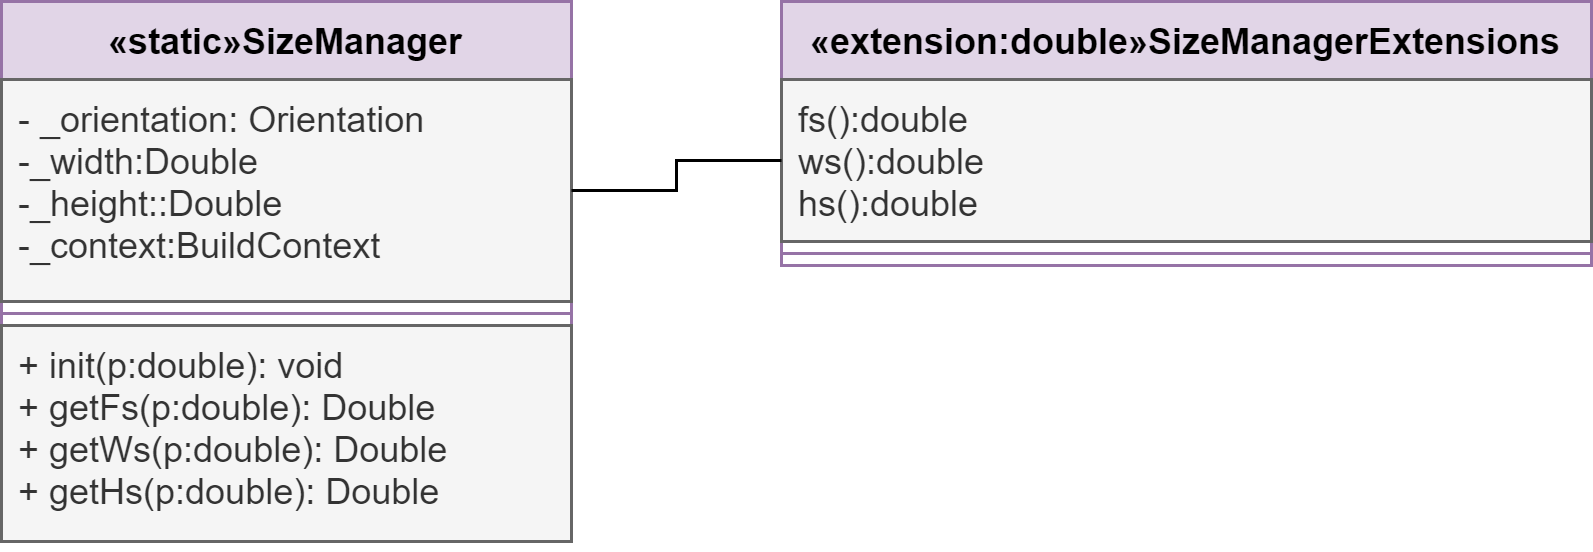
\includegraphics[width=1\textwidth]{FLUTTER/images/GP/SizeManagerKlassen.png}
\caption{Klassendiagramm des SizeManagers}
\end{figure}

\newpage
\subsubsection{Expanded Widget}
 Ein Expanded Widget ermöglicht die Ausdehnung eines Elements, um die gesamte verfügbare Höhe bzw. Breite zu verwenden. Teilen sich mehrere Widgets eine Zeile bzw. Spalte, wird der verfügbare Raum gleichermaßen aufgeteilt.
\begin{lstlisting}[caption=Eine Reihe mit zwei gleich breiten Buttons,style=goMono]
SizedBox(
        height: 7.0.hs,
        child: Row(
          mainAxisAlignment: MainAxisAlignment.spaceEvenly,
          children: [
            Expanded(
              child: CardButton(
                  text: 'Reservieren',
                  onPress: () async {
                    //....
                  }),
            ),
            Expanded(
              child: CardButton(
                  text: 'Jetzt holen',
                  onPress: () async {
                    //....
                  }),
            )
          ],
        ),
      );
\end{lstlisting}

\GpSSec{Theme Handler}\label{subsec:impl:themehandler}
Ein Theme Handler ist für die Verwaltung der Schriftarten, Schriftartengrößen, Farben und jegliche andere Art von Designeigenschaften verantwortlich. \\
Bei der Implementierung der Apps wurde entschieden, einen hellen und dunklen Modus zu integrieren. Dazu wurde eine {\textit{Themeprovider}} Klasse geschrieben, welche das {\textit{Provider}} (details unter \ref{subsec:thero:statemanagement} \nameref{subsec:thero:statemanagement}) Paket bzw. dessen {\textit{notifyListeners()}} Methode verwendet. Bei der {\textit{notifyListeners()}} Methode handelt es sich um eine übersichtlichere und performantere Form des {\textit{Notifier-Patterns}}. Dadurch erspart man sich das Interface für die Benachrichtigungen, falls sich der Zustand des {\textit{Themes}} ändert

\newpage

\begin{lstlisting}[caption=Verwendung ThemeProvider Klasse,style=goMono]
import 'package:flutter/material.dart';
import 'package:card_master/client/config/palette.dart';
import 'package:card_master/client/domain/persistent/app_preferences.dart';

class ThemeProvider extends ChangeNotifier {
  late ThemeMode _themeMode;

  ThemeProvider() {
    _themeMode = AppPreferences.getIsOn() ? ThemeMode.dark : ThemeMode.light;
  }
  void toggleTheme(bool isOn) {
    await AppPreferences.setIsOn(isOn);
    _themeMode = isOn ? ThemeMode.dark : ThemeMode.light;
    notifyListeners();
  }

  ThemeMode getThemeMode() {
    return _themeMode;
  }
}

//main.dart
class RfidApp extends StatelessWidget{
    //......
    @override
    Widget build(BuildContext context) {
    return ChangeNotifierProvider(
      create: (context) => ThemeProvider(),
      builder: (context, \_) {
        final themeProvider = Provider.of<ThemeProvider>(context);
        if (rememberState) {
          return MaterialApp(
            debugShowCheckedModeBanner: false,
            title: title,
            themeMode: themeProvider.getThemeMode(),
            theme: RifdAppThemes.lightTheme,
            darkTheme: RifdAppThemes.darkTheme,
            routes: routes,
            home: const ClientNavigation(),
            navigatorKey: navigatorKey,
          );
        }
}
\end{lstlisting}

\newpage

Wenn der Switch-Button zum Wechseln des Themes gedrückt wird, wird die Methode {\textit{toggleTheme}} aufgerufen, die je nach Zustand des Buttons, eines der unterhalb definierten Themes verwendet. Danach werden alle {\textit{Subscriber}} benachrichtigt, dass sich das Theme geändert hat.\\

Das zuletzt verwendete Theme wird ebenfalls mit der Klasse {\textit{AppPreferences}} gespeichert. Unterhalb der Klasse {\textit{ThemeProvider}} wird das Abonnieren der ThemeProvider Klasse gezeigt. Zunächst muss das Startwidget {\textit{MaterialApp}} ein Kind von dem Widget {\textit{ChangeNotifierProvider}} sein. Die ChangeNotifierProvider Klasse benötigt den Parameter {\textit{create:}}, welcher im Grunde genommen das {\textit{subscribe}} eines {\textit{Notifier Patterns}} darstellt. In der Zeile 30 wird die Instanz von {\textit{ThemeProvider}}, die bei {\textit{create:}} erstellt wurde, zugänglich gemacht. Bei Zeile 35 erfolgt eine Referenzierung auf den {\textit{ThemeMode}} Wert, der verwendet wird.

\begin{lstlisting}[caption=Definiton der App Themes,style=goMono]
import 'package:card_master/admin/config/theme/palette.dart';
import 'package:flutter/material.dart';

class RifdAppThemes {
  //whitemode
  static get darkTheme => ThemeData(
        fontFamily: 'Kanit',
        scaffoldBackgroundColor: Colors.black,
        colorScheme:
            const ColorScheme.dark().copyWith(primary: ColorSelect.blueAccent),
        primaryColor: Colors.white,
        secondaryHeaderColor: ColorSelect.blueAccent,
        dividerColor: ColorSelect.darkBorder,
        cardColor: ColorSelect.darkCardColor,
      );

  //darkmode
  static get lightTheme => ThemeData(
        fontFamily: 'Kanit',
        scaffoldBackgroundColor: ColorSelect.lightBgColor,
        colorScheme:
            const ColorScheme.light().copyWith(primary: ColorSelect.blueAccent),
        primaryColor: Colors.black,
        secondaryHeaderColor: ColorSelect.blueAccent,
        dividerColor: ColorSelect.lightBorder,
        cardColor: ColorSelect.lightCardColor,
      );
}
\end{lstlisting} 

\newpage

\subsubsection{Ablauf – und Klassendiagramm}
\begin{figure}[h!]
\centering
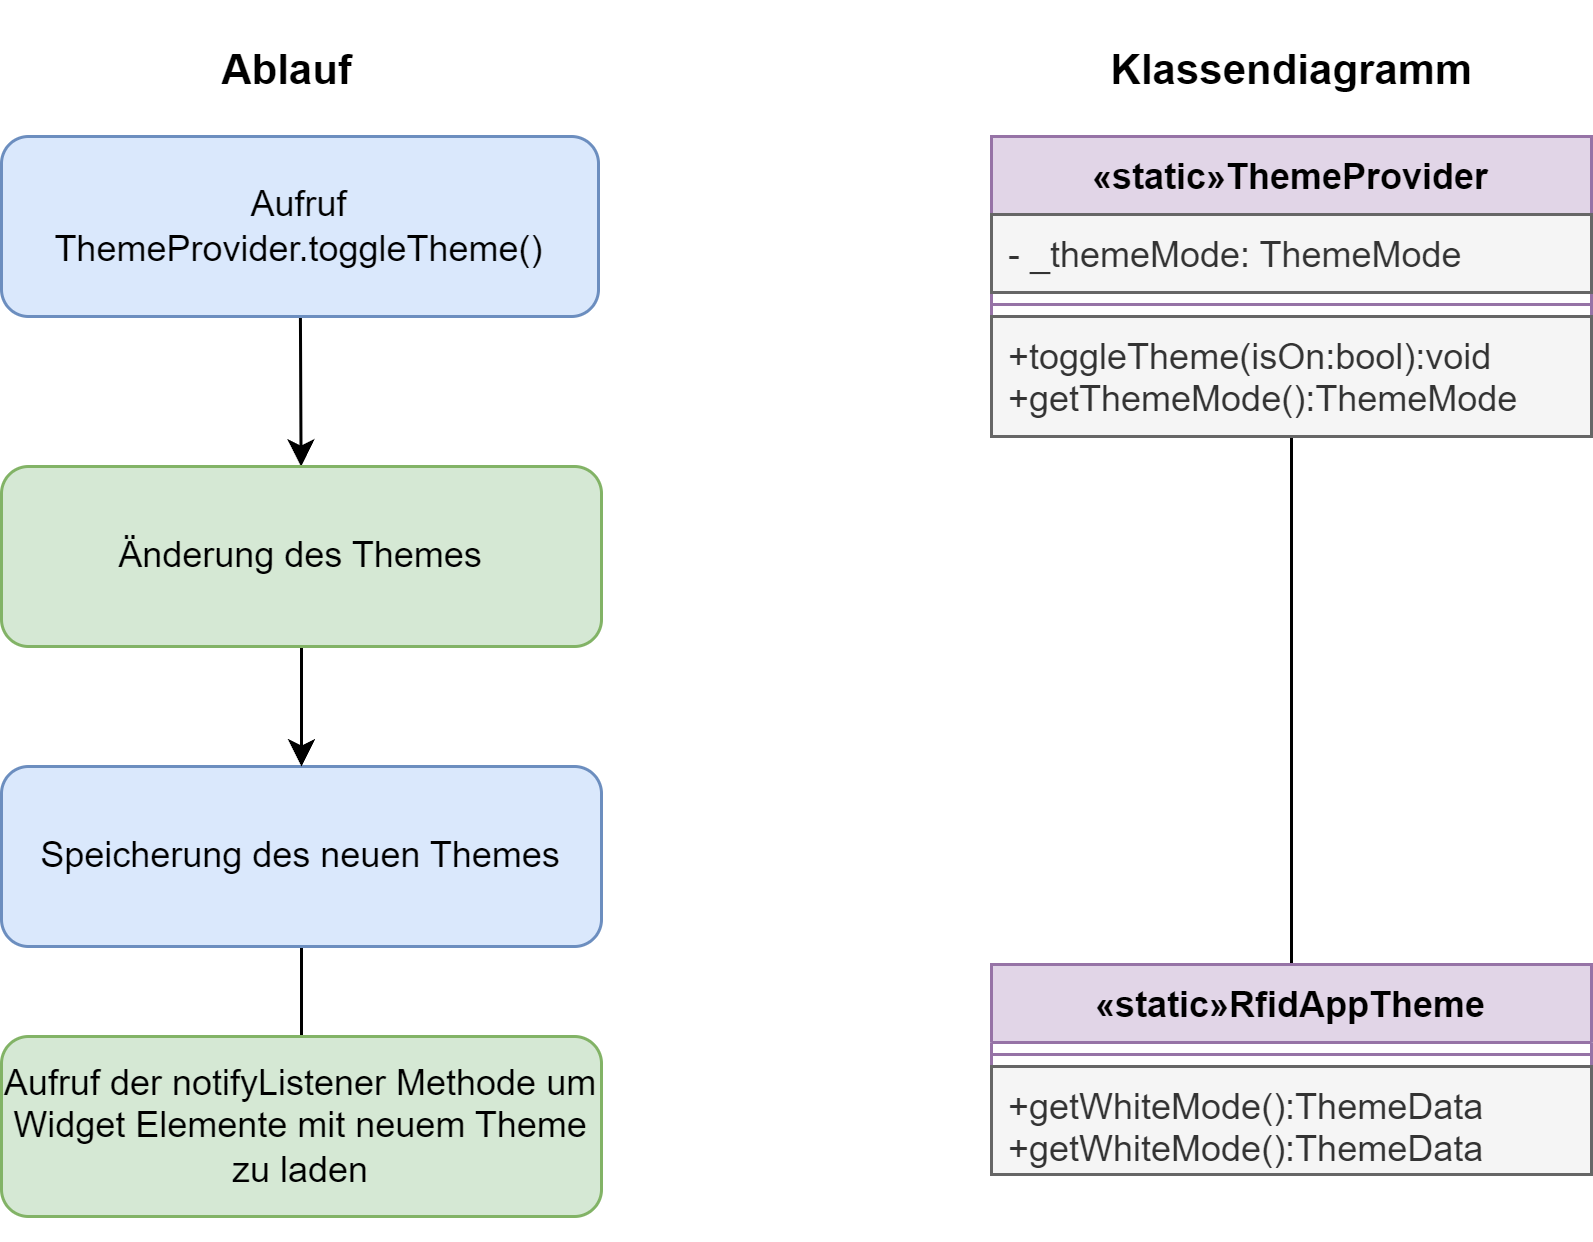
\includegraphics[width=1\textwidth]{FLUTTER/images/GP/ThemeProviderAblauf.png}
\caption{Ablauf - und Klassendiagramm für ThemeProvider}
\end{figure}
\newpage
\GpSSec{Inherited Widget}\label{inheritedwidget}
Bei einem Inherited Widget handelt es sich um ein Konzept in Flutter, welches den Datenaustausch entlang des Widget-Baumes verwaltet, indem genau eine Klasse definiert wird, welche die Daten speichert. Dieses Konzept wurde für die Implementierung gewählt, um teilweise das Definieren von den Funktionsparametern zu vernachlässigen, vor allem wenn ein Eltern-Widget mehrere Kinder-Widgets hat. In der Abbildung \ref{img:klassendiagrammkarten} werden Inherited Widgets verwendet, um Daten zwischen Widgets auszutauschen. Die Erkl\"arung der verschiedenen Arten von Widgets wird im Abschnitt \ref{subsec:thero:widgets} \nameref{subsec:thero:widgets} beschrieben.

\begin{lstlisting}[caption=Beispiel Inherited Klasse,style=goMono]
class CardsData extends InheritedWidget {
    final List<ReaderCard> readercards;
    final String searchstring;
    final Set<String> pinnedCards;
    final void Function() reloadPinned;
    final void Function() reloadCard;
    final void Function(void Function()) setState;
    
    const CardsData({
      Key? key,
      required this.readercards,
      required this.searchstring,
      required this.pinnedCards,
      required this.reloadPinned,
      required this.reloadCard,
      required this.setState,
      required Widget child,
    }) : super(key: key, child: child);
    
    static CardsData? of(BuildContext context) {
      return context.dependOnInheritedWidgetOfExactType<CardsData>();
    }
    
    @override
    bool updateShouldNotify(CardsData oldWidget) {
      return readercards != oldWidget.readercards ||
          searchstring != oldWidget.searchstring ||
          pinnedCards != oldWidget.pinnedCards;
    }
}
\end{lstlisting}

In der Zeile 17 wird das gewünschte Kinder-Widget deklariert. Die Methode {\textit{.of(BuildContext context)}} wird verwendet, um Mithilfe eines BuildContexts das richtige Inherited Widget zurückzugeben. Die {\textit{.updateShouldNotify}} wird dann aufgerufen, wenn sich Daten bei einem Eltern-Widget geändert haben, um die betroffenen Daten bei den Kinder-Widgets neu zu laden.
Um die Daten des Inherited Widget bei einem Kinder-Widget zu verwenden, erfolgt bei der {\textit{.build Methode}} eines Kinder-Widgets eine Referenzierung auf das Inherited Widget über die {\textit{.of}} Methode mithilfe des aktuellen BuildContexts.

\begin{lstlisting}[caption=Referenzierung auf das InheritedWidget \"uber .of Methode,style=goMono]
class CardView extends StatelessWidget {
    //...
    late CardsData cardsData;
    CardView({super.key});
    @override
    Widget build(BuildContext context) {
    cardsData = CardsData.of(context)!;
    return ....
    }
\end{lstlisting}

\newpage
\ZbSSec{Funktionsweise der Navigation}\label{subsec:impl:routes}
Die Navigation der Applikation erfolgt mit dem von Flutter bereitgestelltem Widget
{\textit{BottomNavigationBar}}.
\begin{lstlisting}[caption=Navigation der Client Anwendung,style=goMono]
//represents page
 int currentIndex = 0;
 //all pages of navigation
  final screens = [
    const FavoritePage(),
    const CardPage(),
    const ReservatePage(),
    const SettingsPage()
  ];

  return Scaffold(
        body: screens[currentIndex],
        bottomNavigationBar: BottomNavigationBar(
          type: BottomNavigationBarType.fixed,
          iconSize: 5.0.fs,
          unselectedFontSize: 1.3.fs,
          selectedFontSize: 1.9.fs,
          currentIndex: currentIndex,
          onTap: (value) => setState(() => currentIndex = value),
          backgroundColor: Theme.of(context).scaffoldBackgroundColor,
          selectedItemColor: ColorSelect.blueAccent,
          items: const [
            BottomNavigationBarItem(
              icon: Icon(Icons.favorite),
              label: 'Favoriten',
            ),
            BottomNavigationBarItem(
              icon: Icon(Icons.credit_card),
              label: 'Karten',
            ),
            BottomNavigationBarItem(
              icon: Icon(Icons.info),
              label: 'Reservierung',
            ),
            BottomNavigationBarItem(
              icon: Icon(Icons.settings),
              label: 'Eintellungen',
            )
          ],
        ));
\end{lstlisting}
Dabei werden zunächst alle Seiten der Navigation mit der Liste {\textit{screens}} definiert.Das Scaffold beinhaltet eine {\textit{bottomNavigationBar}}, welche je nach dem Integer {\textit{currentIndex}}, eine andere Seite in der Liste {\textit{screens}} aufruft. Der Parameter {\textit{onTap}} repräsentiert eine Methode, deren primäre Aufgabe in der Änderung des Indexes liegt, wenn ein Element in der BottomNavigationbar gedrückt wird. Der Parameter {\textit{item}}, stellt die angezeigten Icons und Namen der einzelnen Elemente in der Navigationbar dar, wobei das Anordnung mit Definition von {\textit{screens}} sein muss.\\ Eine ausf\"uhrliche Erkl\"arung der {\textit{setState}} Methode ist im Abschnitt \ref{subsec:thero:statemanagement} \nameref{subsec:thero:statemanagement} aufzufinden.

\vspace{1cm}
\begin{figure}[h!]
\centering

\includegraphics[width=0.5\textwidth]{FLUTTER/images/ZB/bottom_navigation.png}
\caption{Navigationsleiste der Client-Sicht}
\end{figure}



\subsubsection{Navigation mit Routen}\label{subsubsec:routes}
Falls das Widget welches im Abschnitt \ref{subsec:impl:routes} \nameref{subsec:impl:routes} nicht verwendet wird, erfolgt der Wechsel der Seiten mit {\textit{Routen}}
Die {\textit{routes.dart}} Datei ist bei einem Projekt mit vielen unterschiedlichen Sichten sinnvoll, um eine bessere Übersicht der gesamten Applikation zu haben. Diese Datei definiert eine Map mit Strings als Key-Werte und Sichten als Value-Werte – die {\textit{Routen}}

\begin{lstlisting}[caption=routes.dart Datei für die User Sicht,style=goMono]
final Map<String, WidgetBuilder> routes = {
  "/login": (context) => const LoginUserScreen(),
  "/favoritepage": (context) => const FavoritePage(),
  "/cardpage": (context) => const CardPage(),
  "/reservatepage": (context) => const ReservatePage(),
  "/settingspage": (context) => const SettingsPage(),
  "/accountpage": (context) => const AccountPage(),
  "/clientnavigation": (context) => const ClientNavigation(),
  //....
};
\end{lstlisting}

Diese Map muss bei der {\textit{main.dart}} Datei beim gewünschten Start Widget angegeben werden, um die erstellten Routen im späteren Verlauf verwenden zu können.

\begin{lstlisting}[caption=Angeben der Routen im Wurzelknoten,style=goMono]
return MaterialApp(
    title: title,
    themeMode: themeProvider.getThemeMode(),
    theme: RifdAppThemes.lightTheme,
    darkTheme: RifdAppThemes.darkTheme,
    routes: routes,
    home: const ClientNavigation(),
    navigatorKey: navigatorKey,
  ); 
\end{lstlisting}

Der Aufruf einer anderen Sicht kann wie folgt aussehen, dabei wird der Key-Wert, welcher in der routes.dart Datei festgelegt wurde verwendet, um die dazugehörige Seite aufzurufen.

\begin{lstlisting}[caption=Wechseln auf die Login Seite mithilfe des /login Schlüssels,style=goMono]
Navigator.pushReplacementNamed(context, "/login");
\end{lstlisting}
\GpSSec{API Middleware }\label{subsec:impl:apimiddleware}
Die Verbindung zu der REST-API erfolgt mithilfe einer Middleware, welche eine Referenz auf eine Methode und eine Map für Argumente als Übergabeparameter definiert. Die Middleware wird im Projekt verwendet, um bestimme Aktionen bzw. das Überprüfen des Authentifizierungsschlüssels und das Handhaben von Errors vor dem Aufruf der jeweiligen REST-Methode zu ermöglichen.\newpage
\begin{lstlisting}[caption=Middleware zum überprüfen des Tokens vor dem Methoden Aufruf,style=goMono]
static Future<Response?> checkAuthorization({BuildContext? context,required Function function, Map<String, dynamic>? args}) async {
    try {
      Response response;
      if (bearerToken == null) {
        await _generateToken();
      }
      response = (args != null) ? await function(args) : await function();
      if (response.statusCode == 401) {
        await _generateToken();
        response = (args != null) ? await function(args) : await function();
      }
      if (response.statusCode != 200) {
        throw Exception(response.body);
      }
      return response;
    } catch (e) {
      if (context != null) {
        SnackbarBuilder(
                context: context,
                header: "Error",
                snackbarType: SnackbarType.failure,
                content: e.toString())
            .build();
      }return null;}}
\end{lstlisting}

Der Rückgabetyp {\textit{Future<Response?>}} repräsentiert einen asynchronen Vorgang, der ein zukünftiges Objekt vom Typ {\textit{Response}} liefert. Asynchrone Programmierung bzw. Future wird bei Prozessen verwendet, die mehr Zeit wie übliche Operationen benötigen. Ohne der asynchronen Programmierung würde die ganze Anwendung, durch den Aufruf diese Methode blockiert werden. Eine umfangreiche Beschreibung der theoretischen Grundlagen zur asynchrone Programmierung in Flutter ist im Abschnitt beschrieben \ref{subsec:thero:async} \nameref{subsec:thero:async}
Das {\textit{?}} bei {\textit{Response}} gibt an, dass die Rückgabe den Wert {\textit{null}} haben kann, falls Fehler während der Ausführung auftreten.
\begin{itemize}
    \item Ist der Token null, wird ein neuer Token generiert (Zeile 8).
    \item Danach wird die Methode für die API Anfrage bspw. {\textit{getCards}}, je nach Zustand der Argumente (null oder nicht null) ausgeführt Zeile(7).
    \item Ist der Status Code der Anfrage 401 (not authorized), wird ein neuer Token generiert (Zeile 10). Der Status 401 kann durch den Verfall des Tokens z.B nach 2 Stunden oder durch den Wechsel eines Standardbenutzers mit einem registrierten Benutzer eintreten.
    \item Danach wird die benötigte API-Anfrage wieder aufgerufen, dieses Mal authentifiziert (Zeile 11). 
    \item Ist die Anfrage nun ungleich 200 (Anfrage passt, OK) wird eine Exception aufgerufen (Zeile 14). Andernfalls wird die Antwort {\textit{response}} zurückgeben.
    \item Durch das {\textit{catch}} am unteren Teil wird ein Pop-Up mit der jeweiligen Antwort des Servers angezeigt. Es kann aber vorkommen, dass kein Pop-Up angezeigt wird, falls kein {\textit{BuildContext}} übergeben wurde.
\end{itemize}

\newpage

\subsubsection{EPK Diagramm}

\begin{figure}[h]
\centering
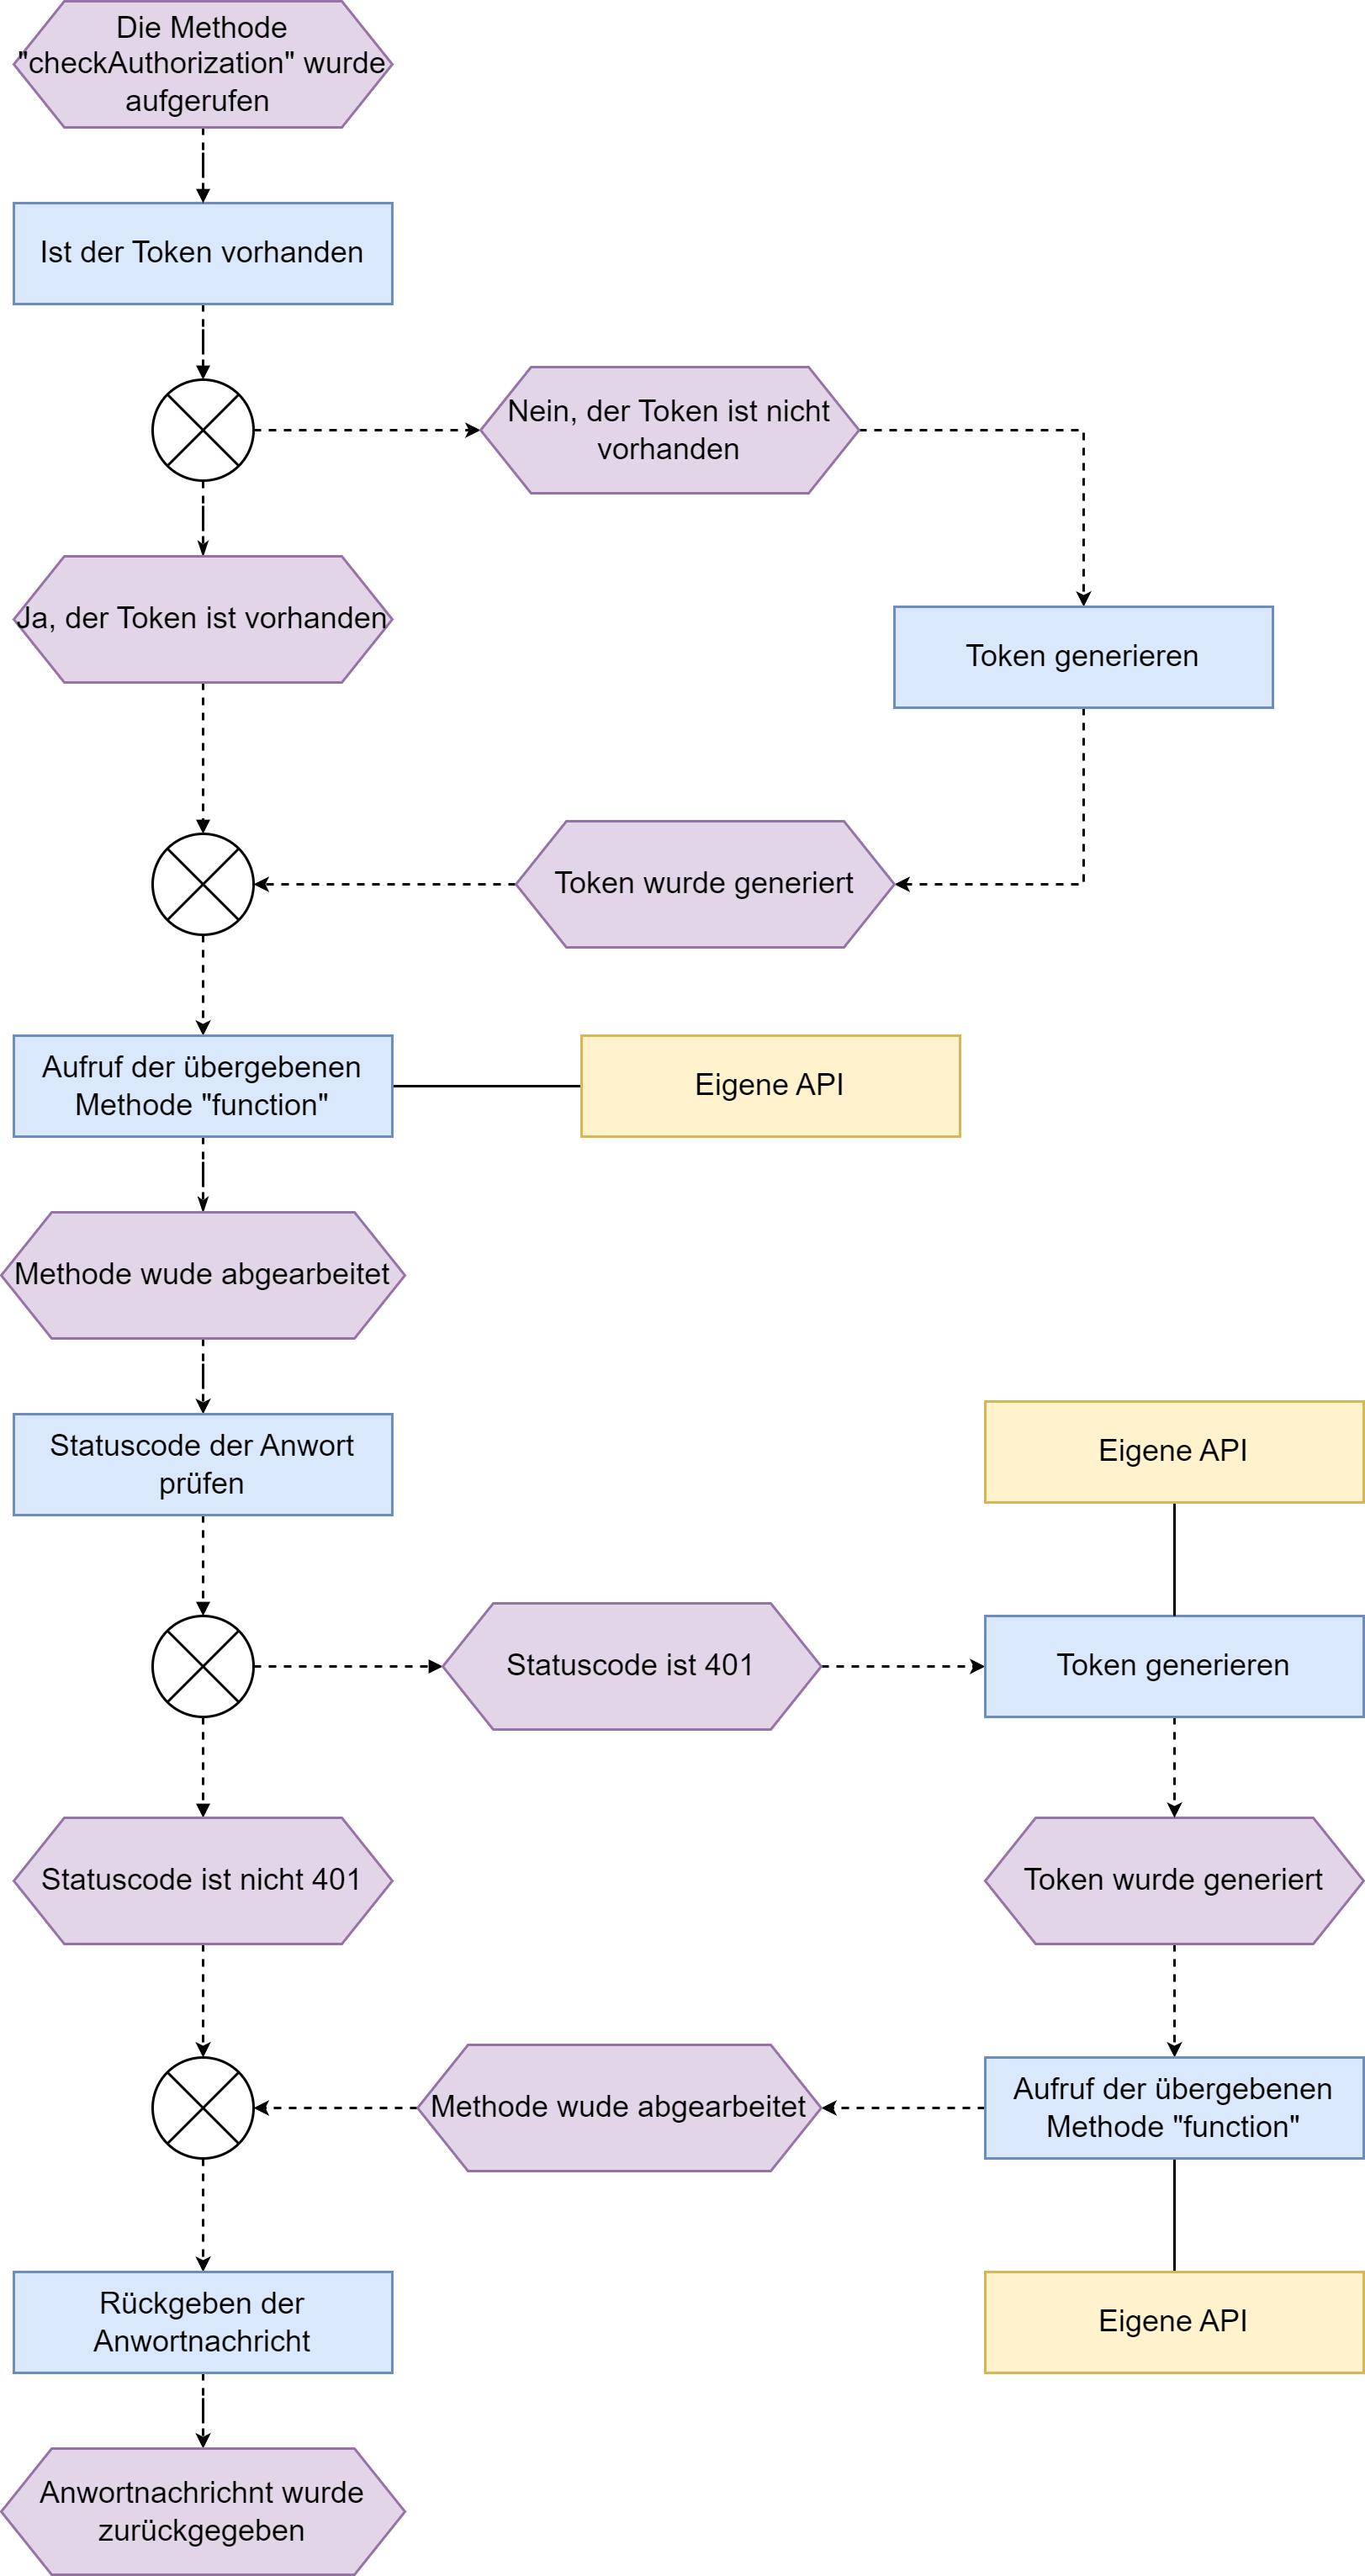
\includegraphics[width=0.52\textwidth]{FLUTTER/images/GP/MiddlewareEPK.png}
\caption{EPK Diagramm für die Middleware Methode}
\end{figure}

\newpage
\GpSSec{Feedback Dialog }\label{feedbackdialog}

Das Anzeigen einer Feedback-Komponente nach der Ausführung einer Aktion informiert den Benutzer über mögliche Fehler bzw. Erfolge. Dies ist vor allem, bei der Feststellung der Ursache eines Misserfolges wichtig.

Für die App wurde festgelegt, die Feedback-Komponente mittels eines Pop-Ups zu realisieren, wobei dessen Auftreten unterschiedliche Gründe haben kann. Der Pop-Up Dialog wird je nach Art der Meldung anders dargestellt
\begin{itemize}
        \item {\textbf{Erfolg:}} Wie der Name schon sagt, wird diese Art von Pop-Up angezeigt, wenn eine Aktion erfolgreich durchgeführt wurde. Beispiele hierfür sind eine erfolgreiche Registrierung oder das Anfordern von Karten.
        \item {\textbf{Hinweis:}} Der Hinweisdialog, wird angezeigt, um den Nutzer auf ein bestimmtes Ereignis aufmerksam zu machen. 

        \item {\textbf{Warnung:}} Der Warnungsdialog wird angezeigt, um den Benutzer auf eine Situation aufmerksam zu machen, die nicht unbedingt ein kritisches Problem darstellt. Fehlende Informationen oder eine fehlerhafte Eingabe seitens des Benutzers stellen eine Warnung dar.


        \item {\textbf{Error:}} Dieser Dialog, wird bei der Unterbrechung einer Aktion durch ein bestimmtes Ereignis angezeigt. Ein weiterer Unterschied zu den anderen Arten ist, dass die gesamte Fehlernachricht ebenfalls beim Dialog angezeigt wird. Beispiele hierfür wären, wenn die Anwendung keine Verbindung zum Server herstellen konnte oder eine {\textit{Exception}} während der Ausführung der Applikation ausgelöst wurde.
\end{itemize}

\begin{figure}[h!]
\centering
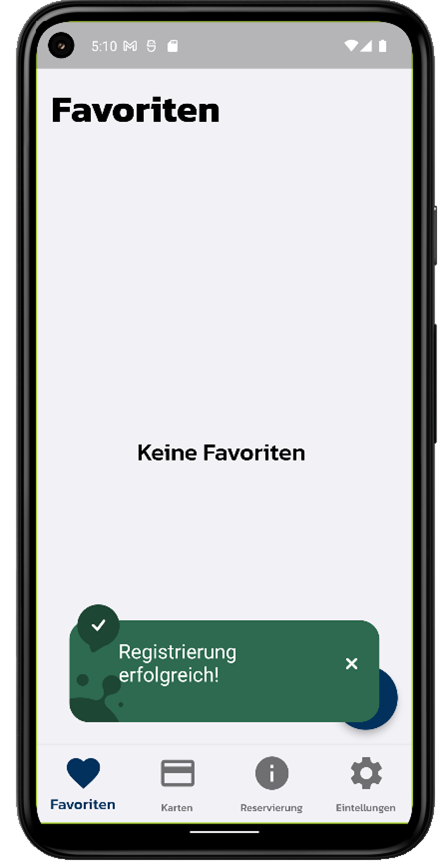
\includegraphics[width=0.28\textwidth]{FLUTTER/images/GP/Login_register_sucees.png}
\caption{Erfolgreiche  Registrierung}
\end{figure}


%\begin{wrapfigure}{r}{0.3\textwidth}
%\centering
%    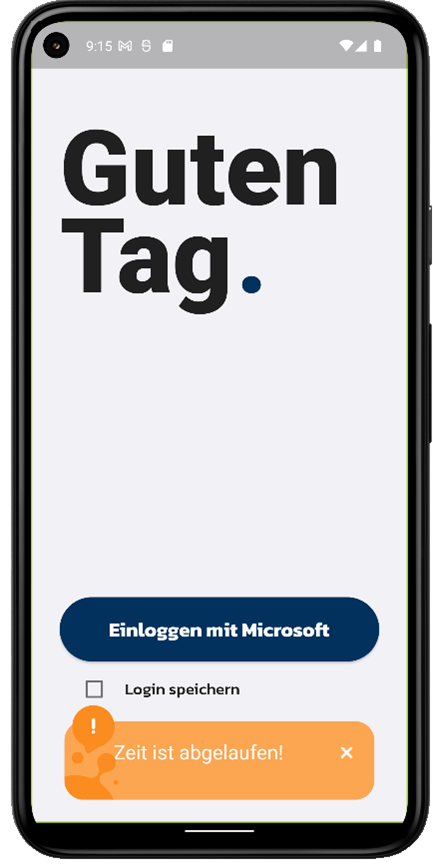
\includegraphics[width=0.18\textwidth]{FLUTTER/images/GP/Login_Error.png}
%    \caption{Warnungsnachricht bei der Registrierung}
%    \label{fig:client_allg}
%\end{wrapfigure}
Die Realisierung des Feedback-Dialogs erfolgt durch das Paket {\textit{awesome\_snackbar\_content}}. Allerdings wurde das Paket etwas umprogrammiert, um unterhalb der \"Uberschrift einen Text anzeigen zu können und die responsive Eigenschaft des Pop-Ups zu erfüllen.
\newpage
\begin{lstlisting}[caption=Feedback Builder Klasse,style=goMono]
class FeedbackBuilder {
  final FeedbackType snackbarType;
  final BuildContext context;
  final String header;
  dynamic content;
  
  FeedbackBuilder(
      {required this.snackbarType, required this.context,
      required this.header, this.content});
      
  void build() {
    SnackBar? snackBar;
    switch (snackbarType) {
      case FeedbackType.success:
        snackBar = SnackBar(
            behavior: SnackBarBehavior.floating,
            content: AwesomeSnackbarContent(
              title: header,
              message: (content == null) ? '' : content.toString(),
              contentType: ContentType.success,
            ));
      case FeedbackType.warning:
\end{lstlisting}

\newpage

Um ein Pop-Up anzeigen zu lassen, benötigt die Klasse, eine Überschrift, den Buildcontext, den Typ (Error, Warnung usw.) und optional einen Text. Der Typ des Pop-Ups wird durch das Enum {\textit{Feedbacktype}} realisiert. Bei der Methode 'build()' wird je nach Enum ein unterschiedliches Pop-Up erstellt. Insgesamt gibt es 4 {\textit{Feedbacktypen}}: success, help, warning, failure, wobei jeder Typ einer der vorhin erklärten Arten von Meldungs-Nachrichten entspricht.  
\begin{lstlisting}[caption=Awendung des FeedbackBuilders bei einer Exception,style=goMono]
try{
//...
} catch (e) {
if (context != null) {
    FeedbackBuilder(
        context: context,
        header: "Error",
        snackbarType: FeedbackType.failure,
        content: e.toString())
    .build();
}
\end{lstlisting}


\GpSSec{Darstellung der API Daten}\label{subsec:impl:visualizeapidata}

\subsubsection{Deserialisierung }
Um die Daten, die von der API übertragen werden, in eine Struktur zu verwandeln, welche von der Anwendung verstanden wird, erfolgt eine Deserialisierung der Informationen. Hierbei wird die {\textit{JSON-Tree}} Struktur in Data Transfer Objects (DTOs) umgewandelt, welche im späteren Verlauf für die  Verarbeitung und Anzeige von Daten auf der Benutzeroberfläche verantwortlich sind. Den theoretischen Hintergrund zu der Deserialisierung finden Sie im Abschnitt \ref{subsec:thero:deserialization} \nameref{subsec:thero:deserialization} bzw. \ref{subsubsec:thero:dtos} \nameref{subsubsec:thero:dtos}
\newpage
\begin{lstlisting}[caption=\"Ubertragungsdaten eines Storages in Form von JSON,style=goMono]
[
    {
        "name": "S4",
        "location": "L4",
        "address": "1.1.1.1",
        "capacity": 10,
        "cards": [
            {
                "reader": "0X3LH0BB-RI=",
                "name": "KarteEingangshalleSued",
                "position": 0,
                "accessed": 4,
                "available": false,
            },
        ]
    }
]
\end{lstlisting}
Die nachfolgende DTO Klasse beschreibt das Wurzelelement {\textit{Storage}}. Diese Klasse beinhaltet nach der Deserialisierung, die Namen/Werte Paare der JSON Nachricht.
\begin{lstlisting}[caption=Dto Klasse Storage,style=goMono]
class Storage {
  String name;
  String location;
  String address;
  int capacity;
  List<ReaderCard> cards;

  @override
  Storage(
      {required this.name, required this.location,
      required this.address, required this.capacity,
      required this.cards});
      
  factory Storage.fromJson(dynamic json) {
    var cardsObjJson = json['cards'] as List;
    List<ReaderCard> cards =cardsObjJson.map((tagJson) => ReaderCard.fromJson(tagJson)).toList();
    return Storage(
        name: json["name"],
        location: json['location'],
        address: json['address'],
        capacity: json['capacity'],
        cards: cards);
  }
}
\end{lstlisting}
Die Funktion 'Storage.fromJson' erhält die JSON-Daten der API-Antwort (siehe Abschnitt \ref{subsec:impl:apimiddleware} \nameref{subsec:impl:apimiddleware}) als Parameter und konvertiert sie je nach Typ in eine weitere DTO-Klasse (Zeile 18) oder in ein Attribut wie beispielsweise 'name'. Das Schlüsselwort 'factory' gibt an, dass die Methode eine Instanz der Klasse erstellt und zurückgibt.
%i moch ds eh 


\subsubsection{Darstellung der deserialisierten Daten }

Die Darstellung der Karten, welche mittels der {\textbf{REST-API}} bereitgestellt bzw. deserialisiert werden, erfolgt über einen {\textit{FutureBuilder}}. Ein FutureBuilder ist ein Widget der Flutter SDK, um asynchrone Vorgänge zu verarbeiten und anzuzeigen. Wie der Name schon sagt, erwartet der FutureBuilder, Daten vom Typ Future, welche von der Middleware der API deserialisiert und geliefert werden. Der theoretische Hintergrund zur asynchronen Programmierung ist im Abschnitt \ref{subsec:thero:async} \nameref{subsec:thero:async} aufzufinden

\begin{lstlisting}[caption=Vereinfachte Darstellung eines FutureBuilders,style=goMono]
 FutureBuilder<List<ReaderCard>?>(
              //Future Objekt vom Typ Future<ReaderCards>
              future: readerCards,
              builder: (context, snapshot) {
                  //Hier finden Fehlerbehandlung statt
                  //...
                  //Date der API
                  final cards = snapshot.data!;
                  switch (site) {
                    case CardPageType.Karten:
                      return CardsData(
                        //Parameter....
                        child: CardView(),
                      );
                    case CardPageType.Favoriten:
                      return CardsData(
                        //Parameter....
                        child: FavoriteView(),
                      );

                    case CardPageType.Reservierungen:
                      return CardsData(
                        //Parameter....
                        child: ReservationView(),
                      );
                  }
                }
                return const Text("Error");
              }),
\end{lstlisting}
  {\textbf{Hinweis:}} CardPageType ist eine Enum, die kennzeichnet, welche Informationen bei den Karten in der GUI angezeigt werden sollen. In diesem Beispiel gibt es drei unterschiedliche Arten, eine solche Karte aufzubauen. 
  
    Mittels des Aufrufs {\textit{snapshot.data}}, können die Daten, welche vom asynchronen (\ref{subsec:thero:async} \nameref{subsec:thero:async}) Vorgang entstanden sind, geladen werden. In diesem Fall wird eine Liste des Typs ReaderCards angefordert. Diese Daten werden je nach Typ von {\textit{CardPageType}} an ein Widget weitergeleitet, welches diese Daten interpretiert, auswertet und in den einzelnen {\textit{Karten}} f\"ur die GUI visualisiert. Um Codeverdoppelung zu minimieren wurde jeweils eine Wrapper Klasse für Admin und Client Sicht erstellt, deren primäre Aufgabe darin besteht, die API-Daten abzurufen (\ref{subsec:impl:apimiddleware} \nameref{subsec:impl:apimiddleware}) und diese in einem FutureBuilder zu verwenden.{\textbf{Wrapper Klassen}} beschreiben ein Konzept der objektorientierten Programmierung. Die Verwendung solch einer Klasse in Flutter, beschreibt ein Widget, welches ein anderes Widget umschließt, um zusätzliche Funktionalitäten oder dessen Darstellung zu ändern. 

\begin{figure}[h!]
\centering
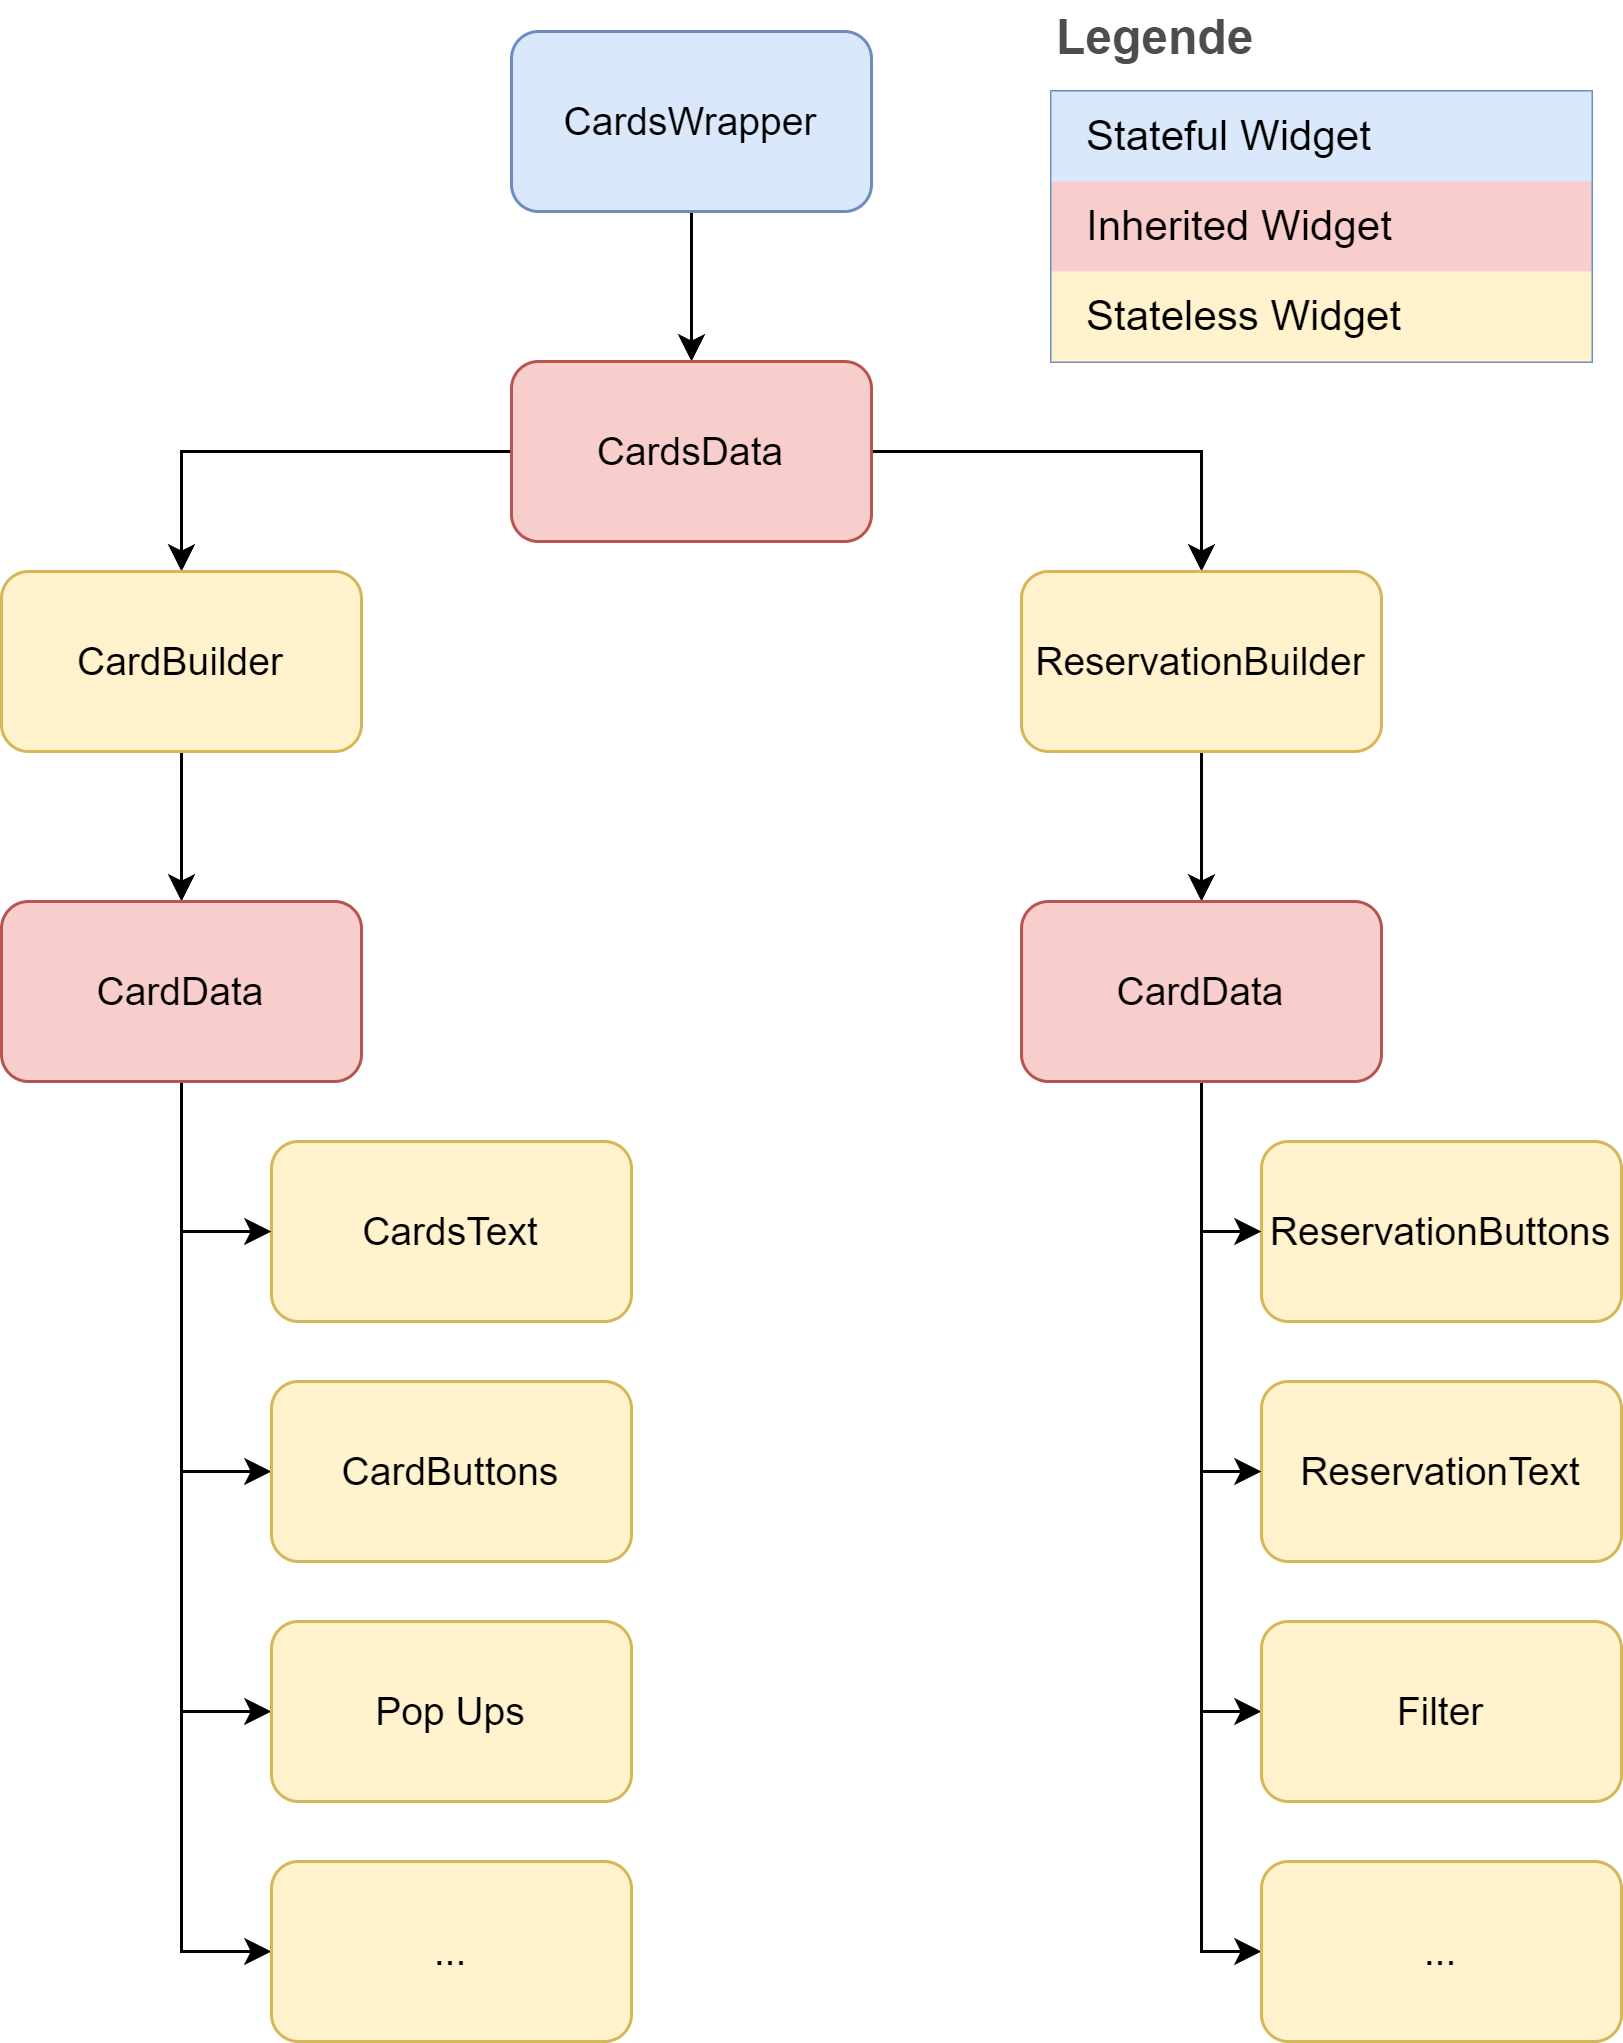
\includegraphics[width=0.5\textwidth]{FLUTTER/images/GP/structure_inherited.png}
\caption{Klassendiagramm für Erstellung Karten}
\label{img:klassendiagrammkarten}
\end{figure}
\newpage
   

\GpSSec{Anmeldungsablauf }\label{subsec:impl:login}
Der Registrierungsvorgang beinhaltet, das Anmelden mittels Microsoft und das darauffolgende Scannen der Karte eines Nutzers. Ebenfalls ist es m\"oglich den Login zu speichern, damit die Abfrage der Benutzerdaten, bei erneuter Verwendung der App nicht mehr notwendig ist. Die Anleitung zur Registrierung ist im Abschnitt \ref{sec:userguider:loginview} \nameref{sec:userguider:loginview} aufzufinden.
\\
Die Anmeldung über Microsoft erfolgt mit dem Paket {\textit{aad\_oauth}}, welches  die Möglichkeit gibt, die Authentifizierung der Identität des Benutzers über das {\textit{Azure Active Directory}} zu integrieren. Ebenfalls kann mit dem AAD geprüft werden, ob es sich nun wirklich um eine Lehrkraft des Linzer Technikums handelt. Wenn die Anmeldung des Benutzers über Microsoft erfolgreich war, wird ein Token zur Verfügung gestellt, der  die Möglichkeit gibt, die Daten des Benutzers über die {\textit{Microsoft Graph API}} abzufragen. Der Vorteil der Implementierung dieses Prozesses besteht darin, dass kein Passwort mehr benötigt wird, was das Sicherheitsrisiko der Anwendung enorm verringert.

\subsubsection{Login Handler}
Die {\textit{handleSignIn}} Methode wird beim Anmeldeprozess der Login Sicht jedes Mal bei der Betätigung des Buttons {\textit{Anmelden mit Microsoft}} ausgeführt, sprich bei jeder Anmeldung. Sie überprüft, ob eine Neuregistrierung notwendig ist und führt diese wenn notwendig aus.
\begin{figure}[h!]
\centering
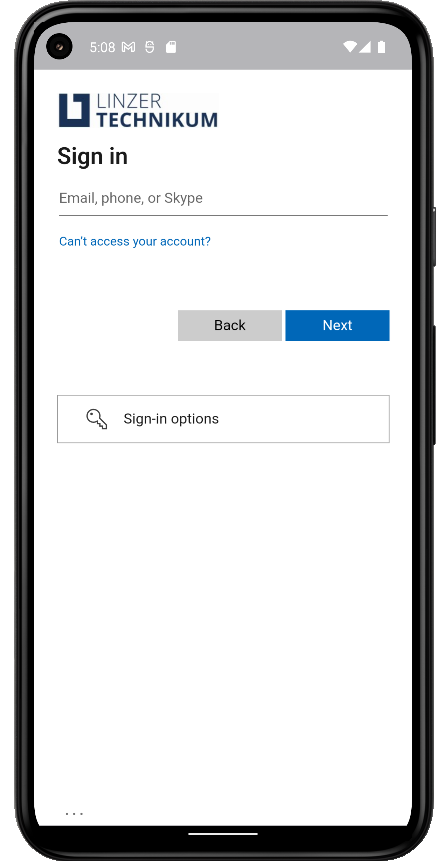
\includegraphics[width=0.2\textwidth]{FLUTTER/images/GP/Login_Micro.png}
\caption{Login mit Microsoft Fenster}
\end{figure}
\newpage

\begin{lstlisting}[caption=\_handleSignIn Methode,style=goMono]
void _handleSignIn() async {
    var loginResult = await UserSessionManager.login(rememberValue);
    if (loginResult == null) return;

     switch (loginResult.item1) {
        case LoginStatusType.REGISTERED:
          Navigator.pushNamedAndRemoveUntil(context, "/clientnavigation", (Route<dynamic> route) => false);
          break;

        case LoginStatusType.NOTREGISTERED:
          if (await UserSessionManager.signUp(
              context, loginResult.item2, rememberValue)) {
            Navigator.pushNamedAndRemoveUntil(
                context, "/clientnavigation", (Route<dynamic> route) => false);
          }
          break;
        case LoginStatusType.ERROR:
          FeedbackBuilder(context: context,header: "Error",snackbarType: FeedbackType.failure,content:loginResult.item2).build();
          break;
      }
  }
\end{lstlisting}

\subsubsection{Ist der Nutzer in unserem System?}
\begin{itemize}
    \item Die Methode UserSessionManager.login ist asynchron (\ref{subsec:thero:async} \nameref{subsec:thero:async}), da sie verschiedene API-Anfragen ausführt. Der Rückgabewert der Methode enthält den Status, der angibt, ob eine Neuregistrierung erforderlich ist und verschiedene Informationen des zu anmeldenden bzw. registrierenden Benutzers.  
   \item Falls, ein Wert zurückgegeben wurde, wird das erste Element des {\textit{Tuples}}, in ein Switch Statement gegeben, um zu sehen, ob der Benutzer bereits registriert ist oder nicht. 
    \item Bei dem Enum  {\textit{LoginStatusType}} {\textit{REGISTERED}}, wird bekannt gegeben, dass der Nutzer bereits im System eingepflegt wurde. Somit erfolgt eine direkte Weiterleitung auf die Client-Sicht 
    \item Falls der Benutzer noch nicht registriert ist ({\textit{NOTREGISTERED}}), wird der Prozess {\textit{UserSessionManager.signUp}} gestartet, um die Neuregistrierung durchzuführen.
    \item Wenn ein Fehler (ERROR) bei der Anmeldung aufgetreten ist, wird ein Pop-Up mit der entsprechenden Fehlermeldung angezeigt.
\end{itemize}

\subsubsection{Ablauf der Login Methode}
\begin{lstlisting}[caption=Methode login in Klasse UserSessionManager,style=goMono]
  static Future<Tuple2<LoginStatusType, dynamic>?> login(bool rememberValue) async {
    try {
      await AadAuthentication.getEnv();
      await AadAuthentication.getOAuth()!.logout();
      await AadAuthentication.getOAuth()!.login();
      String? accessToken = await AadAuthentication.getOAuth()!.getAccessToken();
      if (accessToken!.isEmpty) {
        return null; // Return null if authentication fails
      }
      var microsoftResponse = await Data.getGraphUserData({"accesstoken": accessToken});
      var mircosoftJsonObject = jsonDecode(microsoftResponse.body);
      var email = mircosoftJsonObject["mail"];

      var apiUserResponse = await Data.checkAuthorization(function: Data.getUserByName, args: {"email": email});
      var apiJsonObject = jsonDecode(apiUserResponse.body);
      if (apiJsonObject["email"].toString().isEmpty) {
        return Tuple2(LoginStatusType.NOTREGISTERED, mircosoftJsonObject);
      }
      UserSessionManager.fromJson(apiJsonObject, mircosoftJsonObject);
      if (rememberValue) {
        UserSecureStorage.setUserValues(apiJsonObject, mircosoftJsonObject);
        UserSecureStorage.setRememberState(rememberValue.toString());
      } else {
        UserSecureStorage.setRememberState("false");
      }
      return const Tuple2(LoginStatusType.REGISTERED, null);
    } catch (e) {
      return Tuple2(LoginStatusType.ERROR, e.toString());
    }
  }
\end{lstlisting}
Bei der {\textit{.login} Methode handelt es sich um eine {\textit{asynchrone}} (\ref{subsec:thero:async} \nameref{subsec:thero:async}) Methode, welche ein Future von zwei Objekten {\textit{LoginStatusType und dynamic}} zurückgibt. 

\vspace{0.3cm}
{\textit{LoginStatutsType} ist eine Enum, mit den Typen {{\textit{NOTREGISTERED, REGISTERED oder ERROR}}}. {\textit{Dynamic}} ist ein optionaler Rückgabewert, welcher falls verwendet, die API-Antwort repräsentiert.\\ 

{\textit{Tuple}} ist ein zusätzliches Paket, welches es ermöglicht mehr, als zwei Objekte ohne der Erzeugung einer Liste zurückzugeben. Ebenfalls bekommt die Methode den bool {rememberValue} mit übergeben, welcher je nach Status der {Eingeloggt bleiben} Checkbox die Daten am Gerät speichert oder nicht.
\begin{itemize}
    \item Zunächst wird das Fenster zum Darstellen des Microsoft Logins erzeugt bzw. abgerufen
    \item Falls die Nutzerdaten eingegeben wurden, wird die Methode {\textit{getAccessToken()}} aufgerufen, um den Zugriffstoken zu erhalten.
    \item Falls der Token leer ist, ist die Authentifizierung fehlgeschlagen.
    \item Ansonsten werden mit der Methode {\textit{getGraphUserData}} unter Verwendung des Access Tokens, mit Hilfe der Graph API, die Nutzerdaten abgefragt. Wobei die erhaltenen Daten mit {\textit{jsonDecode}} (\ref{subsec:thero:deserialization} \nameref{subsec:thero:deserialization}) in ein JSON-Objekt umgewandelt werden.
    \item Danach wird mit den erhaltenen Benutzerinformationen der Graph API über die Methode {\textit{getUserByName} }überprüft, ob der Nutzer bereits im System vorhanden ist. Sofern das Feld E-Mail bei Antwort leer ist, wird ein {\textit{Tuple}} mit den Benutzerinformationen und einer Enum LoginStatusType vom Typ {\textit{NOTREGISTERED}} zurückgegeben.
    \item Falls der Nutzer registriert ist werden die Benutzerinformationen mit der Methode {\textit{}{.fromJson}} für die aktuelle Sitzung initialisiert.
    \item Danach werden je nach Zustand des {\textit{rememberValues}} die Benutzerinformationen in einem {\textit{UserSecureStorage}} gespeichert, welcher eine verschl\"usselte Aufbewahrung der Daten am Ger\"art erm\"oglicht
    \item Schlussendlich wird ein {\textit{Tuple}} mit den Benutzerinformationen und ein LoginStatusType vom Typ {\textit{REGISTERED}} zurückgegeben.
    \item {\textbf{Kurz gesagt:}}Je nach Ergebnis der Authentifizierung wird ein entsprechender LoginStatusType zurückgegeben, der angibt, ob der Benutzer bereits angemeldet ist oder ob es sich um einen neuen Benutzer handelt, der sich anmeldet. Wenn während des Ablaufs ein Fehler aufgetreten ist, erscheint ein Dialog (\ref{feedbackdialog}), der die entsprechende Fehlermeldung enthält.
\end{itemize}
\subsubsection{Ablauf der Registrierung}

\begin{lstlisting}[caption= Codeauschnitt der Registrierung,style=goMono]
  static Future<bool> signUp(BuildContext context, dynamic microsoftJsonObject, bool rememberValue) async {
    try {
      await StorageSelectPopUp.build(context);
      if (!StorageSelectPopUp.getSuccessful()) {
        throw ResponseException(FeedbackType.help, "Es wurde kein Storage ausgewaehlt!");
      }
      var reqTimer = RequestTimer(context: context,action: TimerAction.SIGNUP,email: microsoftJsonObject ["mail"],storagename: StorageSelectPopUp.getSelectedStorage());
      await reqTimer.startTimer();
      if (!reqTimer.getSuccessful()) {
        throw ResponseException(reqTimer.getFeedbackType()!, reqTimer.getResponse().toString());
      }
      FeedbackBuilder(context: context,snackbarType: FeedbackType.success,header: "Registrierung erfolgreich!",content: null).build();
      UserSessionManager.fromJson(null, microsoftJsonObject);
      if (rememberValue) {
        UserSecureStorage.setRememberState(rememberValue.toString());
        UserSecureStorage.setUserValues(null, microsoftJsonObject);
      }
      return true;
    } catch (e) {
      if (e is ResponseException) {
        FeedbackBuilder(context: context,snackbarType: e.feedbackType,header: "Registrierung gescheitert!",content: e.toString()).build();
      } return false; } }
\end{lstlisting}

{\textbf{Ablauf:}}
\begin{itemize}
    \item Zun\"achst wird ein Pop-Up mit der Methode {\textit{StorageSelectPopUp.build}} erstellt, welches die Auswahl des Schließfaches, für das Scannen der Karten erm\"oglicht. Die Methode ist asynchron,daher wird das Schlüsselwort await verwendet, um auf die Fertigstellung der Methode zu warten, bevor der Code fortgesetzt wird.
    \item Falls kein Tresor zur ausgew\"ahlt wurde, wird der Registrationsprozess beendet und eine eigens erstellte Exception {\textit{FeedbackException}}, welche für das Anzeigen von Fehlernachrichten  zuständig ist aufgerufen.
    \item Ansonsten, wird ein {\textit{Timer}} gestartet, welcher dem Backend mitteilt, dass ein Registrationsprozess gestartet wird und die restliche Zeit zum Scannen der Karte anzeigt.
    \item Falls die Karte nicht gelesen wurde oder ein anderes Problem aufgetreten ist, wird der Timer unterbrochen und das Flag {successful} auf false gesetzt, um hinzuweisen, dass ein Problem aufgetreten ist. Somit wird eine {\textit{FeedbackException}} aufgerufen und der Registrationsprozess wird unterbrochen.
    \item Ansonsten, werden die Benutzerinformationen mit der Methode {\textit{}{.fromJson}} für die aktuelle Sitzung initialisiert bzw. deserialisiert.
    \item Danach werden je nach Zustand des {\textit{rememberValues}} die Benutzerinformationen in einem {\textit{UserSecureStorage}} gespeichert
    \item Die Methode gibt den Wert {\textit{true}} zurück, um der Methode {\textit{handleSignIn}} zu signalisieren, dass die Neuregistrierung erfolgreich abgeschlossen wurde. Dadurch wird der Benutzer auf die Client-Seite weitergeleitet.
\end{itemize}
\newpage
\subsubsection{EPK Diagramm}
\begin{figure}[h!]
\centering
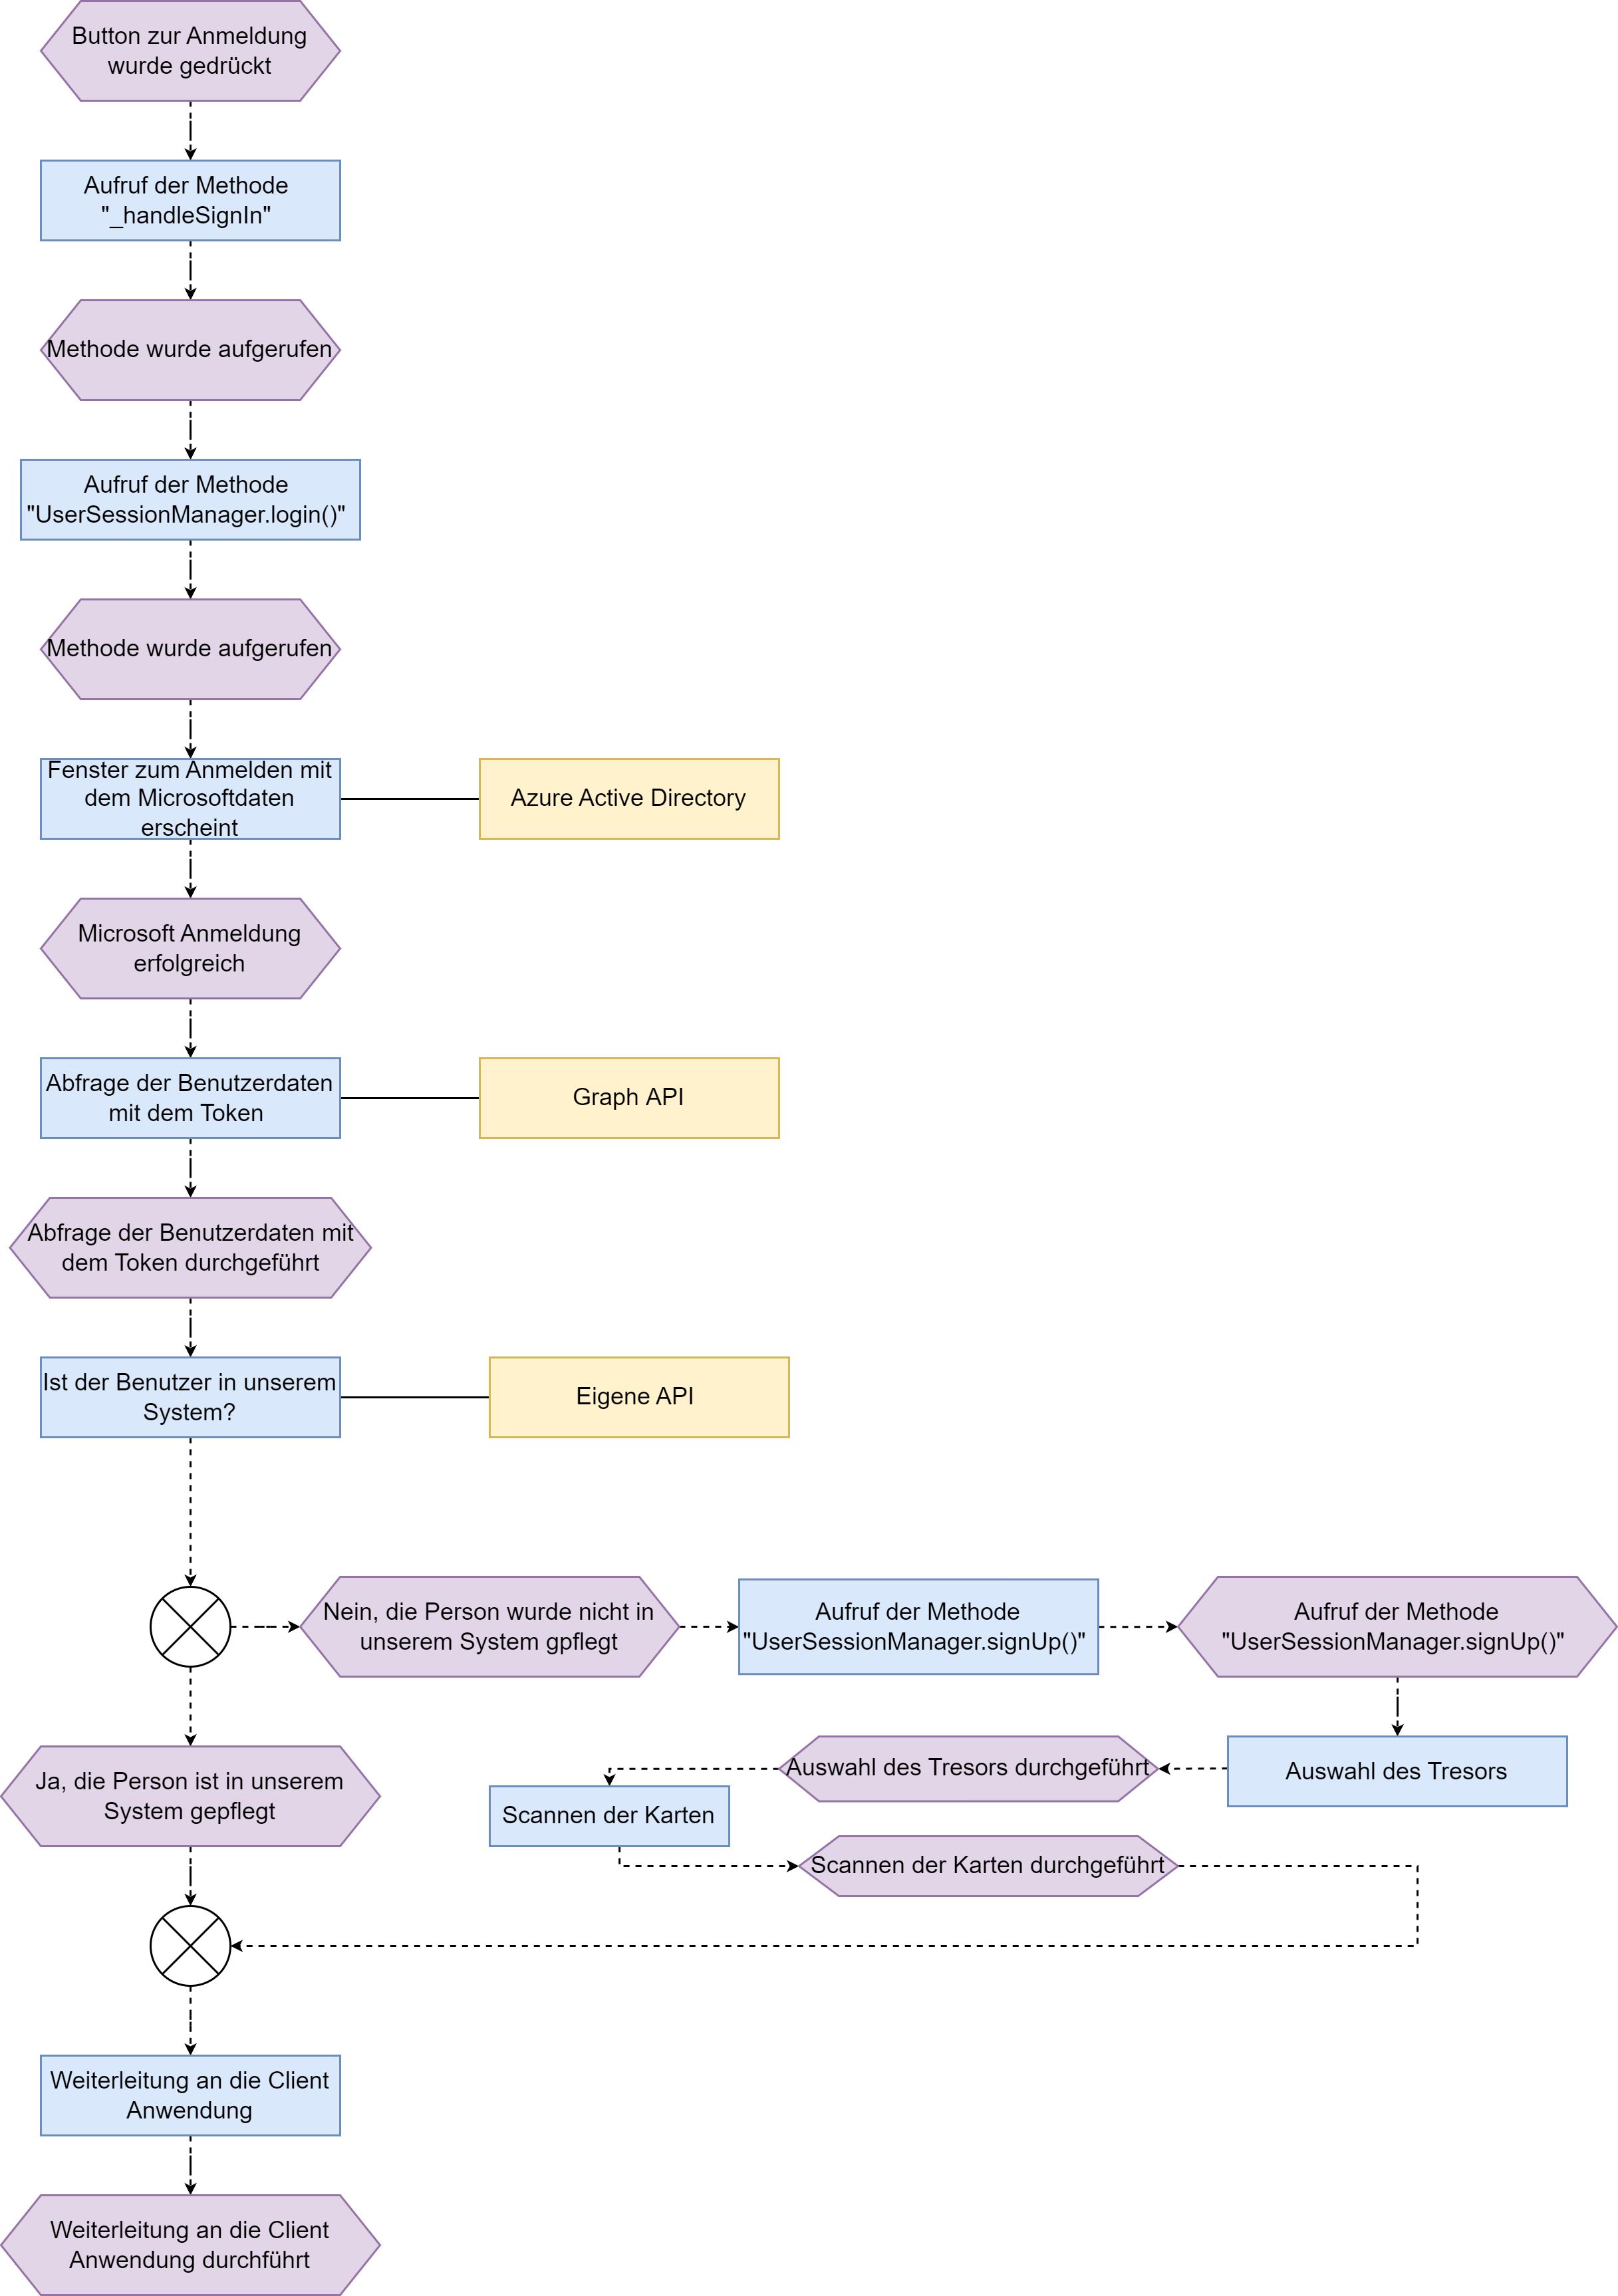
\includegraphics[width=0.82\textwidth]{FLUTTER/images/GP/LoginAblaufEPK.png}
\caption{EPK Diagramm Anmeldung bzw. Registrierung}
\end{figure}

\newpage


\ZbSSec{Timer}\label{subsec:impl:timer}
\begin{wrapfigure}{r}{0.3\textwidth}
\centering
    \includegraphics[width=0.18\textwidth]{FLUTTER/images/GP/Login_timer.png}
    \caption{Timer bei Registrationprozess}
    \label{fig:client_allg}
\end{wrapfigure}
Wie bereits vorhin erwähnt wurde, wird bei verschiedenen Prozessen, wo eine RFID Karte gescannt wird, ein Timer angezeigt. Verwendet wird eine überarbeitete Version des Paktes {\textit{awesome\_snackbar\_content}}.
\\
Dieser Timer dient dazu, eine Anfrage an die API zu senden und die verbleibende Zeit anzuzeigen, die benötigt wird, um die Karte an das Lesegerät am Tresor zu halten, z.B für die Authentifizierung oder das Hinzufügen einer Karte. Abhängig von der Art des Fehlers wird der Klasse ein unterschiedlicher Typ (FeedbackType) zugewiesen, der bestimmt, welche Art von Pop-Up-Fenster angezeigt wird. In dem Pop-Up-Fenster wird dann eine entsprechende Fehlermeldung sowie der Feedback-Typ angezeigt, der über die entsprechenden get-Methoden abgerufen werden kann. Dadurch erhält der Benutzer klare Rückmeldungen über den Status und die Fehler der durchgeführten Aktionen.

Wenn eine Karte gescannt wurde, sendet die API über ein {\textit{Websocket}} eine Nachricht an alle verbundenen Geräte. Dadurch wird der Timer unterbrochen, um nicht mehr die restliche verbleibende Zeit anzuzeigen.
\begin{lstlisting}[caption=Lauschen der Nachrichten vom Websocktet,style=goMono]
_websocketListener() {
    _websocket!.stream.listen((message) async {
      var response = jsonDecode(message);
      _successful = response!["successful"];
      _responseData = response.toString();
      _feedbackType =(_successful) ? FeedbackType.success : FeedbackType.failure;
      channel!.sink.close();
      Navigator.of(context).maybePop();
    }
}
\end{lstlisting} % Wir ham 165 Seiten
\begin{itemize}
    \item Diese Methode überwacht mit {\textit{\_websocket!.stream.listen}}, ob eine Nachricht über den Websocket gesendet wurde.
    \item Sofern eine Nachricht gesendet wurde, wird mithilfe von {\textit{}{jsonDecode}}, die Nachricht deserialisiert.
    \item Danach wird das Attribut {\textit{\_successful}} basierend auf der Nachricht des Websockets aktualisiert, um anzuzeigen, ob das Scannen der Karte erfolgreich war oder nicht.
    \item Außerdem wird die Nachricht des Websockets dem lokalen String {\textit{\_responseData}} zugewiesen. Abhängig davon, ob das Lesen erfolgreich war oder nicht, wird die Variable {\textit{\_feedbackType}} aktualisiert, um den Typ des Pop-Up-Fensters zu bestimmen, der später angezeigt wird.
    \item Zu guter Letzt, wird die Verbindung zum Websocket beendet, und das Pop-Up des Timers geschlossen
\end{itemize}
